\documentclass[intlimits, 9pt, unicode]{beamer}

\mode<presentation>
\usepackage[T2A]{fontenc}
%\usepackage[cp1251]{inputenc}
\usepackage[utf8]{inputenc}
\usepackage[russian]{babel}
\usepackage{graphicx}
\usepackage{amssymb}
\usepackage{amsthm}

\usefonttheme[onlymath]{serif}
\newcommand{\textblue}[1]{\textcolor{blue}{#1}}

\usepackage{beamerthemesplit}

\usetheme{Warsaw}
%\setbeamertemplate{page number in head/foot}[totalframenumber]

\setbeamercovered{transparent}
\beamertemplatenavigationsymbolsempty

\setbeamertemplate{footline}{%
\hfill \insertframenumber{}/\inserttotalframenumber\ \ \ \ }

%\setbeamerfont{footline}{series=\bfseries}
%\setbeamertemplate{footline}[frame number]

\title{Deciphering internet traffic patterns}
\author{Nina Golyandina, Kliment Merzlyakov}
\institute{Saint Petersburg State University \\
     Statistical modeling department \\
    Airpush
}
\date{
    Unlock customer lifetime value with advanced statistical techniques\\
    London\\
    17.10.2018
}

\AtBeginSection[]{
  \begin{frame}
  \vfill
  \centering
  \begin{beamercolorbox}[sep=8pt,center,shadow=true,rounded=true]{title}
    \usebeamerfont{title}\insertsectionhead\par%
  \end{beamercolorbox}
  \vfill
  \end{frame}
}


\begin{document}

\begin{frame}
    \titlepage
\end{frame}

\begin{frame}
    \frametitle{Content}
    
    

    \begin{itemize}
    	\item Change point detection. General notes
    \vspace{0.5cm}
	    \item Mobile advertising data
    \vspace{0.5cm}
        \item Change point detection techniques
    \vspace{0.5cm}
        \item Applications to real data
    \end{itemize}


\end{frame}



\section{Change point detection. General notes}

% \begin{frame}
%     \frametitle{Example}
%
%         \begin{figure}
%         \centering
% 	\textbf{Volume of ads served for specific country}
%         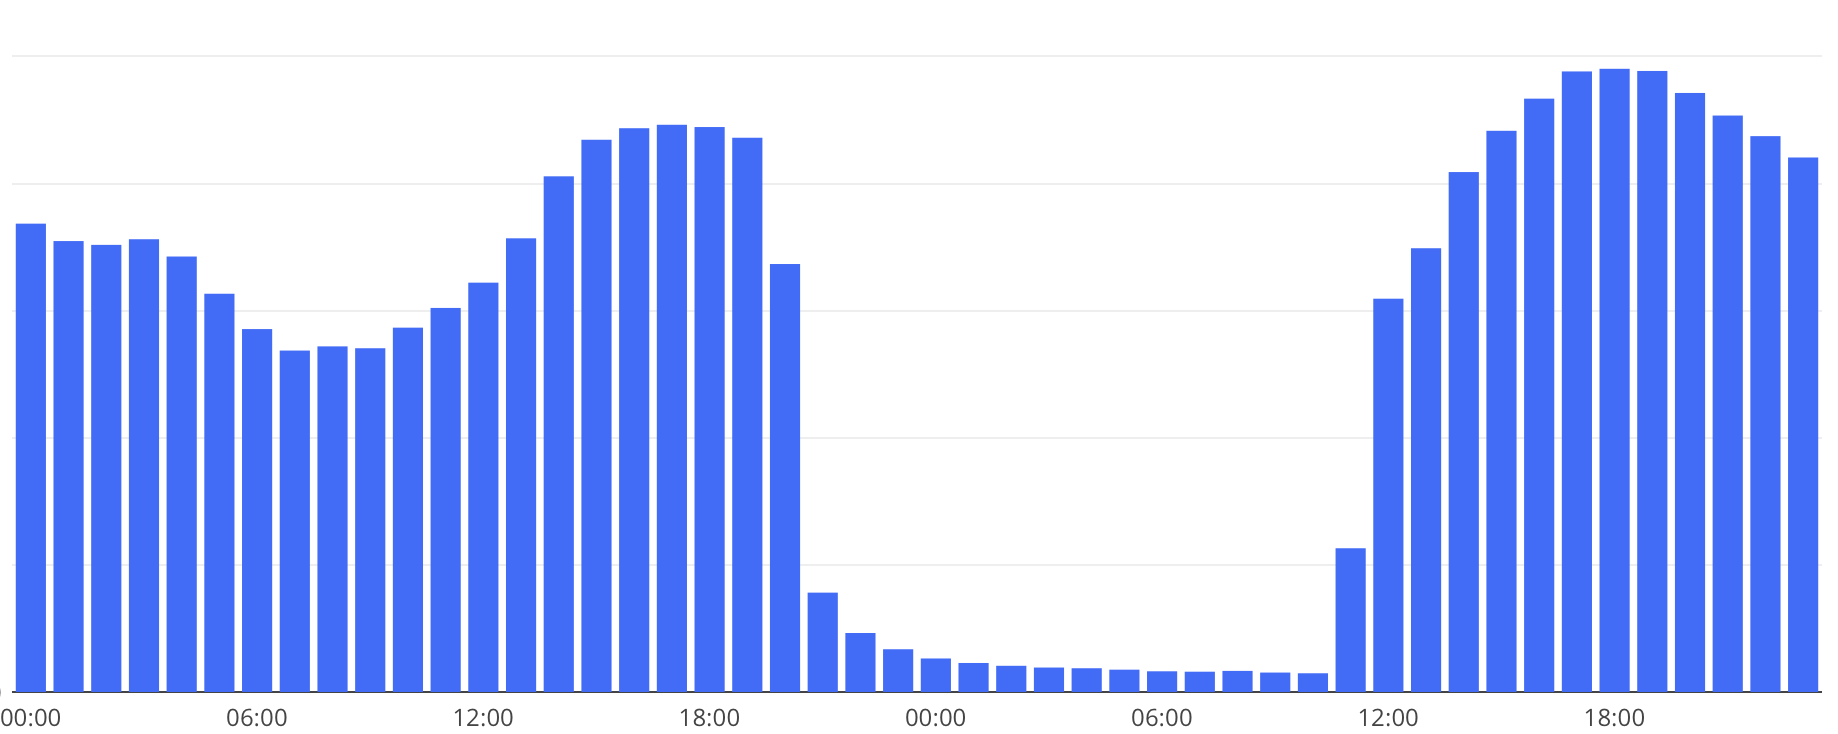
\includegraphics[height=4.5cm]{images/introduction_example}
% 	\end{figure}
	
%     \begin{itemize}
%     	\item Evening change of advertising software
% 	\item Fixed only at morning
% 	\item It's important to detect it automatically and correct it
%     \end{itemize}
% \end{frame}


\begin{frame}
    \frametitle{Changes in data}
    
       \begin{columns}
    \begin{column}{0.25\textwidth}
    \centering
     Request
     \begin{figure}
	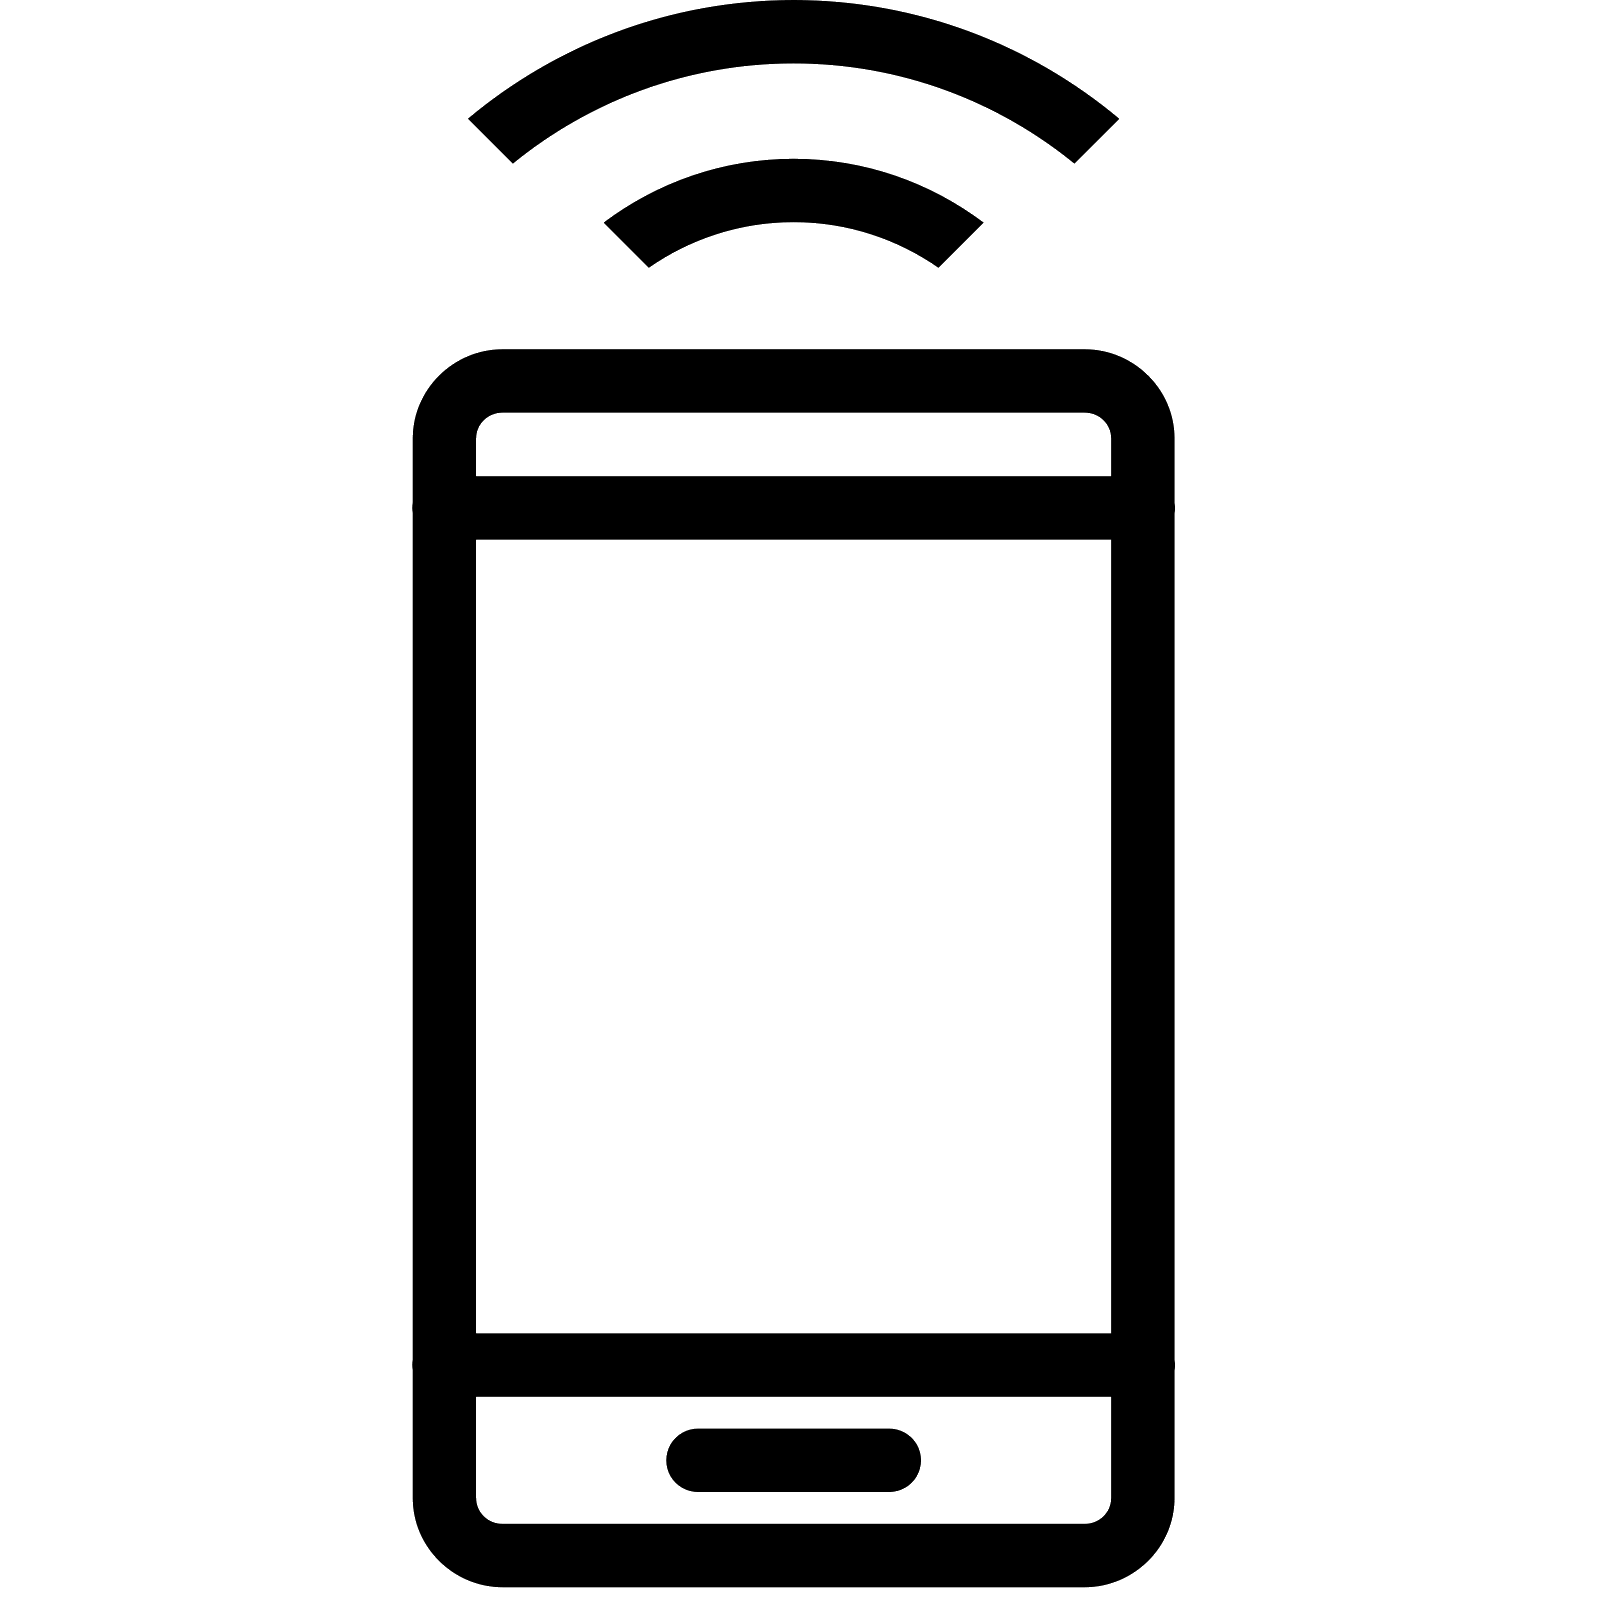
\includegraphics[height=1cm]{images/scheme_request}
     \end{figure}
     \end{column}
    \begin{column}{0.001\textwidth}
    \centering
	>
     \end{column}
    \begin{column}{0.25\textwidth}
    \centering
    Impression
     \begin{figure}
	
\includegraphics[height=1cm]{images/scheme_impression}
     \end{figure}
    \end{column}
    \begin{column}{0.001\textwidth}
    \centering
    >
    \end{column}
    \begin{column}{0.25\textwidth}
    \centering
    Click
     \begin{figure}
	
\includegraphics[height=1cm]{images/scheme_click}
     \end{figure}
    \end{column}
    \begin{column}{0.001\textwidth}
    \centering
    >
    \end{column}
    \begin{column}{0.25\textwidth}
    \centering
     Conversion
     \begin{figure}
	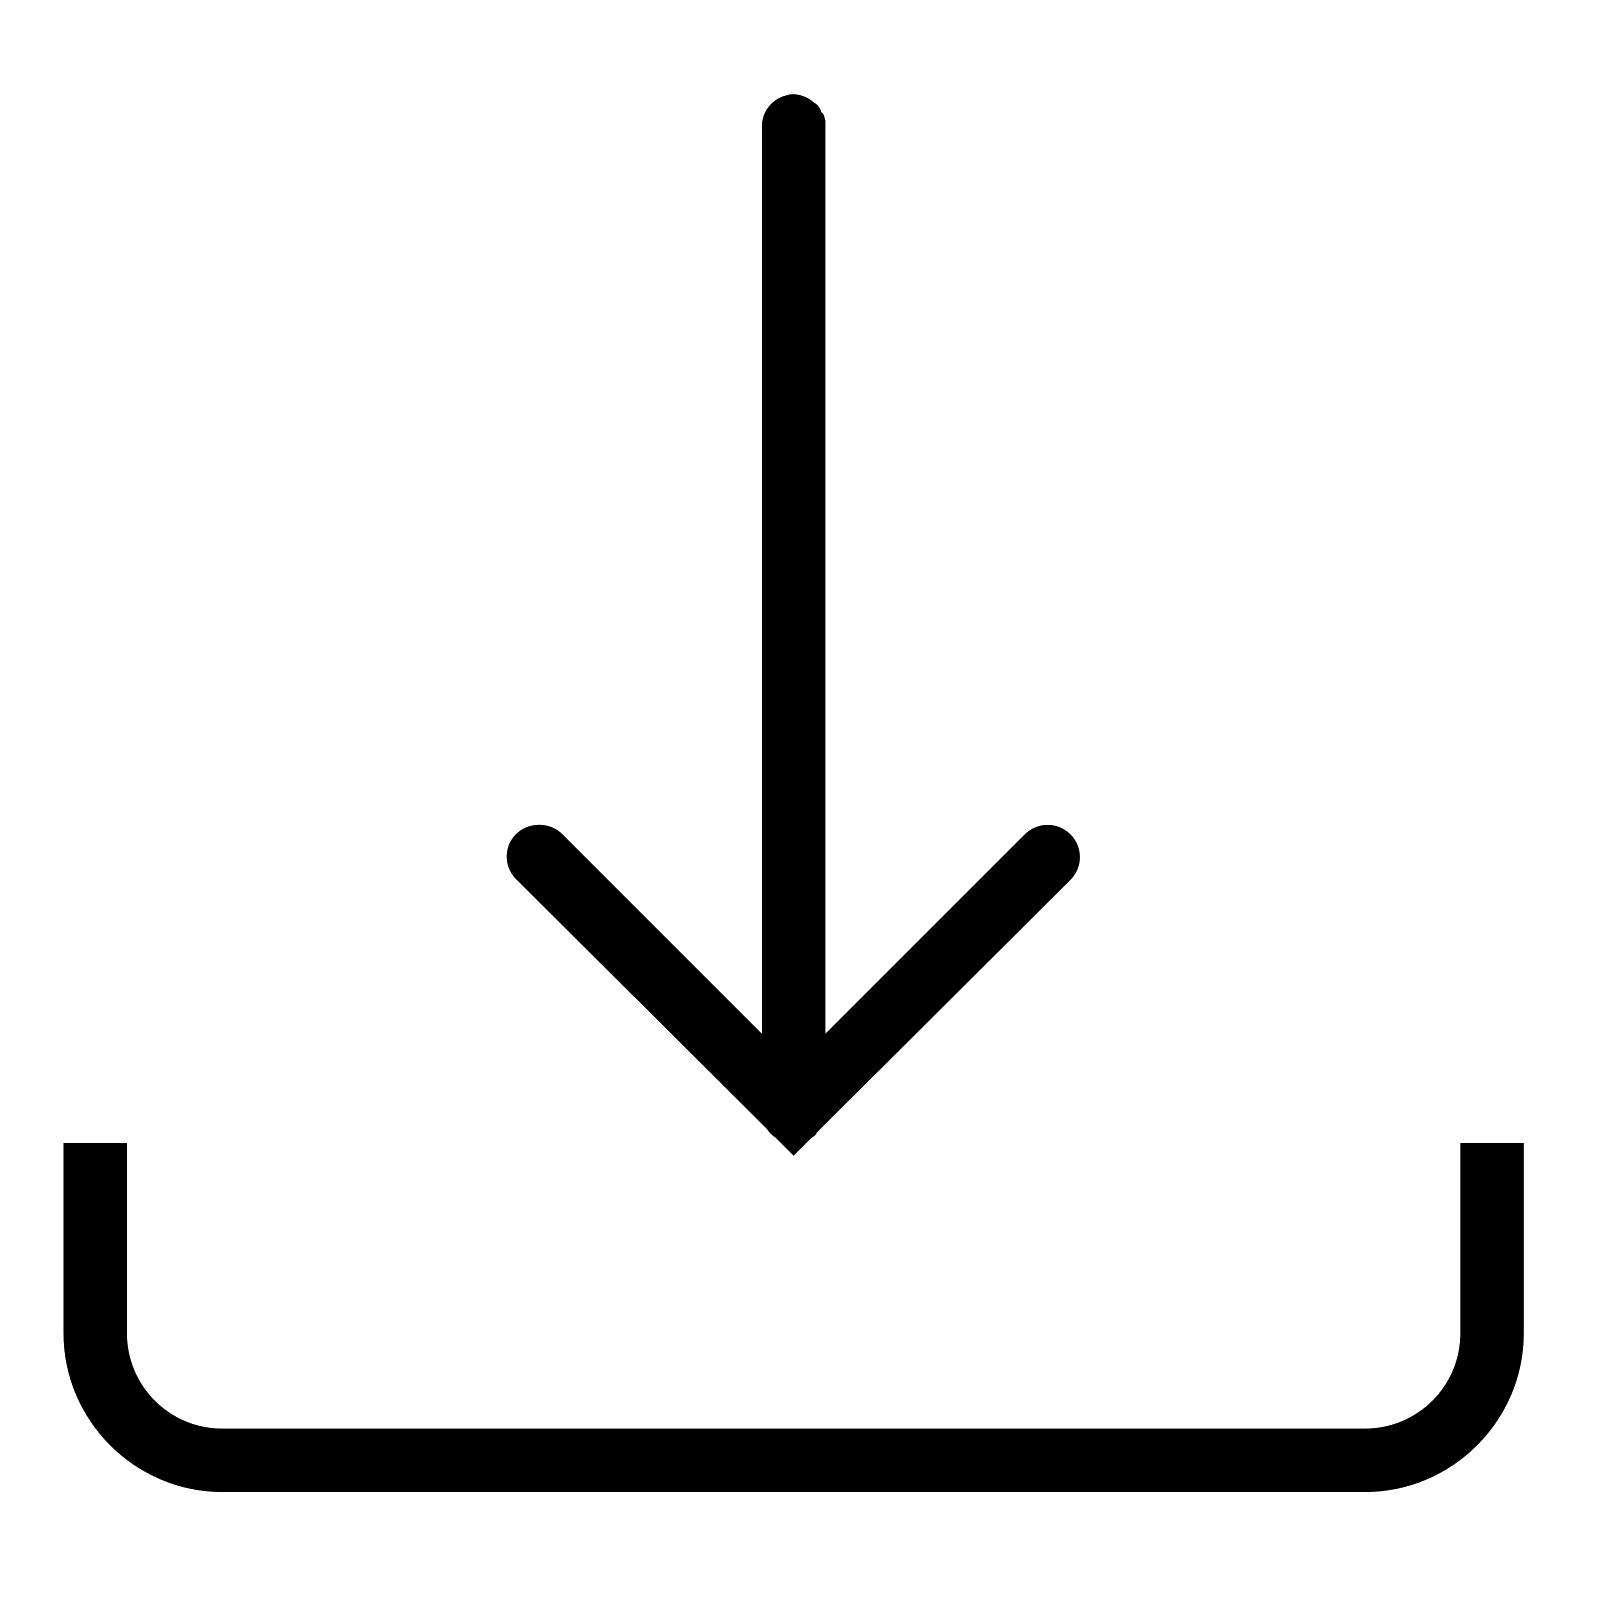
\includegraphics[height=1cm]{images/scheme_conversion}
     \end{figure}
     \end{column}
     \end{columns}
     
             \vspace{1.2cm}

       {\begin{columns}
        \begin{column}{5cm}
        User side changes
         \begin{itemize}
    		\item Application popularity
		\item Competition
		\item Applications' marketing activity
		\item ...
   	 \end{itemize}
        \end{column}
        
        \begin{column}{5cm}
        Advertising network side changes
         \begin{itemize}
    		\item New features released
		\item New advertisers onboarded
		\item New targeting strategy
		\item ...
   	 \end{itemize}
	 \end{column}
    \end{columns}}

 \end{frame}


\begin{frame}
    \frametitle{Time series}
	
    {\begin{columns}
        \begin{column}{5.5cm}
 Time series is a series of values of a quantity obtained at successive times,\\ often with equal intervals between them (minute, hour, day, week, etc.)

\vspace{0.3cm}
\begin{table}[h!]
\centering
 \begin{tabular}{||c c||}
 \hline
 Time & Data \\ [0.5ex]
 \hline\hline
 17-Oct-2018 19:00 & 435 098 \\
 \hline
 17-Oct-2018 20:00 & 431 248  \\
 \hline
 17-Oct-2018 21:00 & 420 329  \\
 \hline
 ... & ... \\ [1ex]
 \hline
\end{tabular}
\end{table}

	
\vspace{0.3cm} Formal notation:
 $ X = (x_1, x_2, ... , x_{N-1} , x_N)  $

        \end{column}

\hspace{-0.5cm}
        \begin{column}{5cm}
Commonly time series can be decomposed $X = T + S + E$
        \begin{figure}
        \centering
	\textbf{Time series. Decomposition example}
        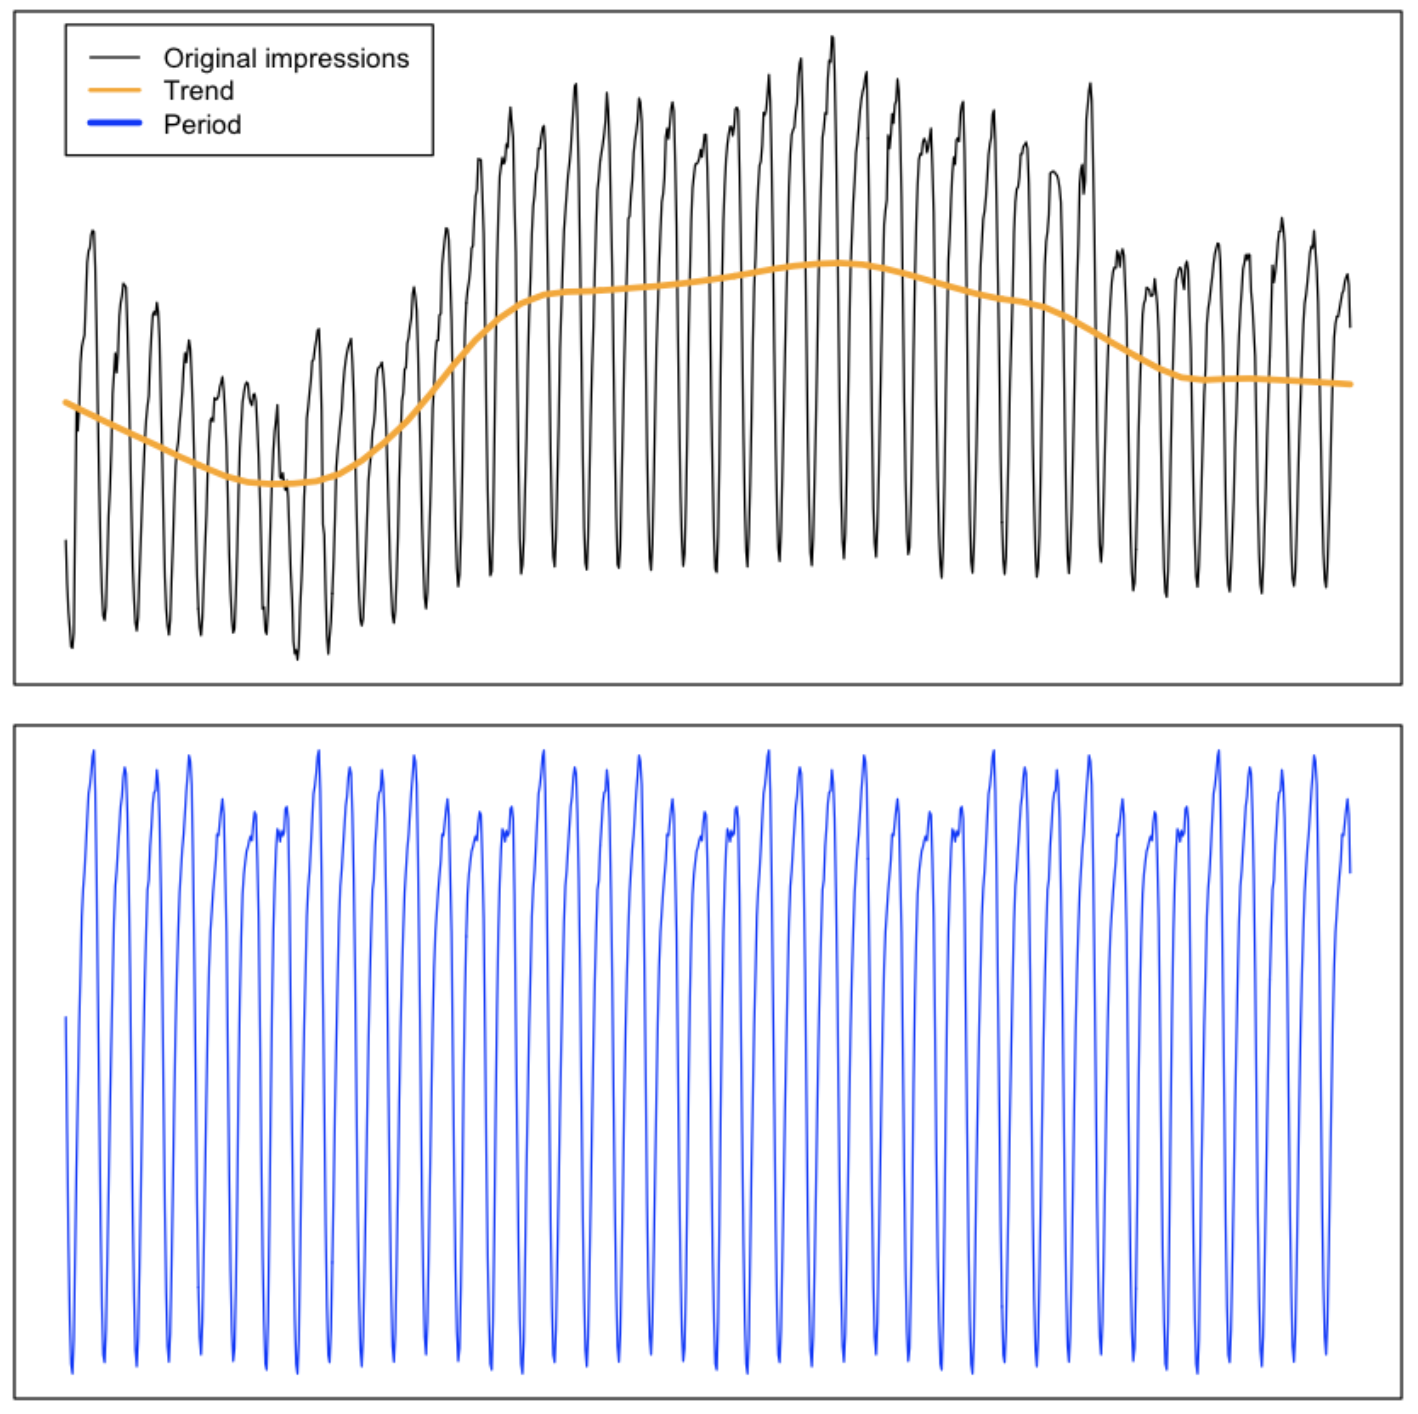
\includegraphics[height=5cm]{images/impressions_stl_3}
	\end{figure}
	
        \end{column}
    \end{columns}}
\end{frame}

\begin{frame}
    \frametitle{What is change point detection?}

    \begin{itemize}
    	\item Change point is a point in time series, where some significant change in structure occurred
	\item Change point detection is a group of methods to find change points in time series
	\item Change points can be of two types:
		\begin{itemize}
			\item Local --- anomaly or outlier
			\item Global --- change of time series structure
		\end{itemize}
    \end{itemize}

    {\begin{columns}
        \begin{column}{5cm}
        \begin{figure}
        \centering
	\textbf{Local change}
        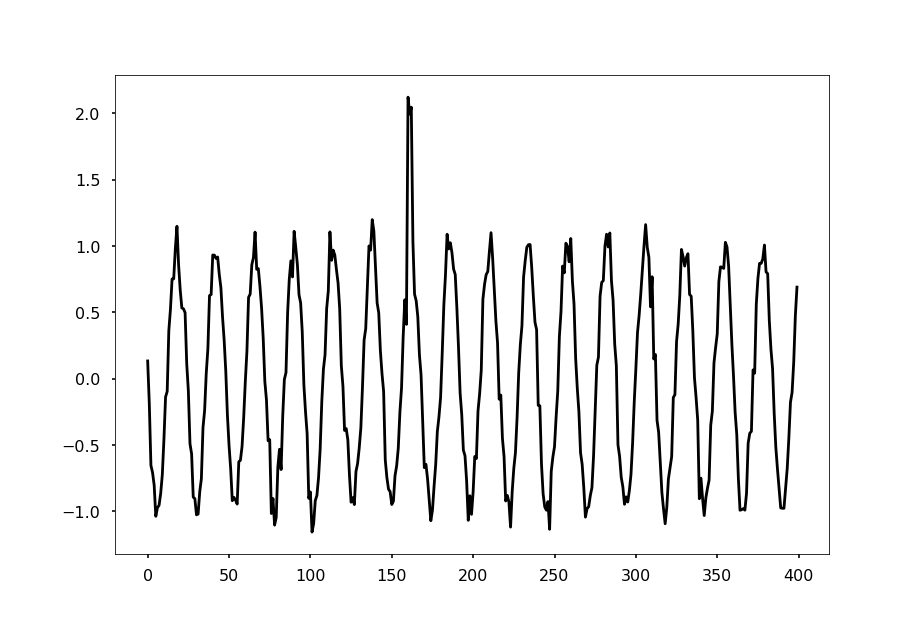
\includegraphics[height=3.5cm]{images/local_cp}
	\end{figure}
        \end{column}

        \begin{column}{5cm}
	\begin{figure}
    	\centering
	\textbf{Global change}
        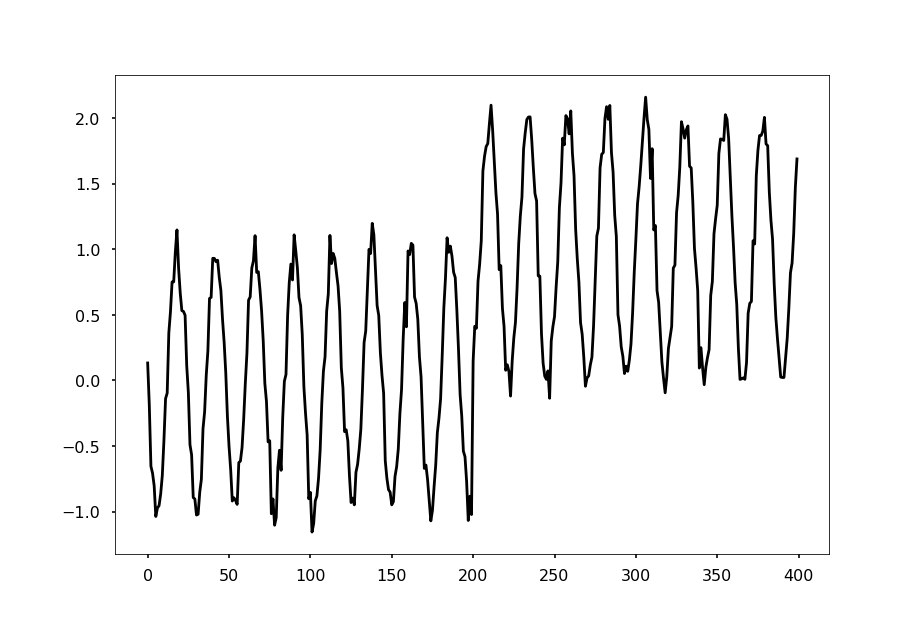
\includegraphics[height=3.5cm]{images/global_cp}
	\end{figure}
        \end{column}
    \end{columns}}

\end{frame}


\begin{frame}
    \frametitle{Motivation}
When it helps:
    \begin{itemize}
    	\item Forecasting
	\item Extracting trend more accurately
    	\item Searching issues in historical data
	\item Reacting on changes quickly
    \end{itemize}


   \begin{columns}
        \begin{column}{5cm}
	\begin{figure}
		\textbf{Without CP detection}
		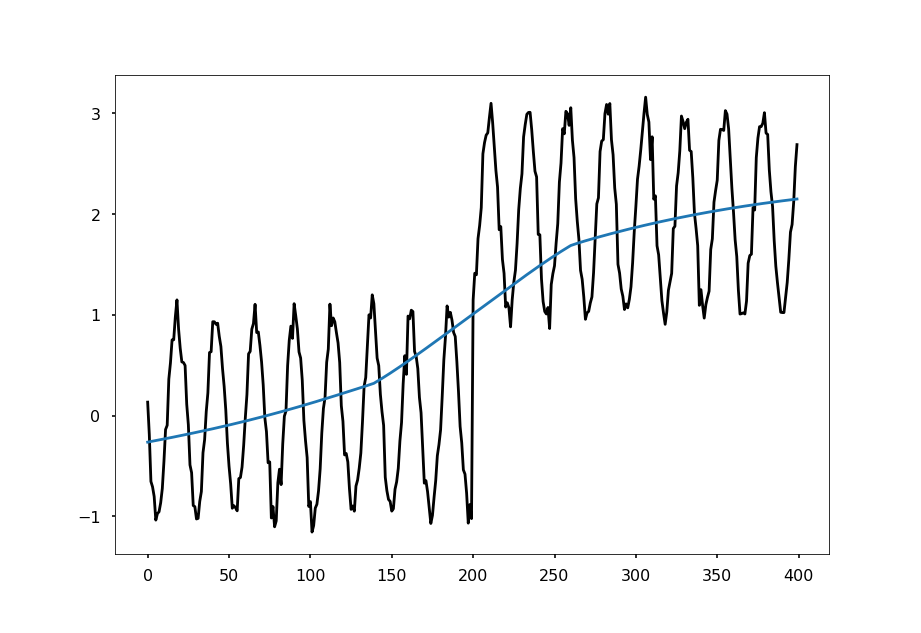
\includegraphics[height=3.5cm]{images/trend_fallacy}
	\end{figure}
        \end{column}

        \begin{column}{5cm}
	\begin{figure}
		\textbf{With CP detection}
		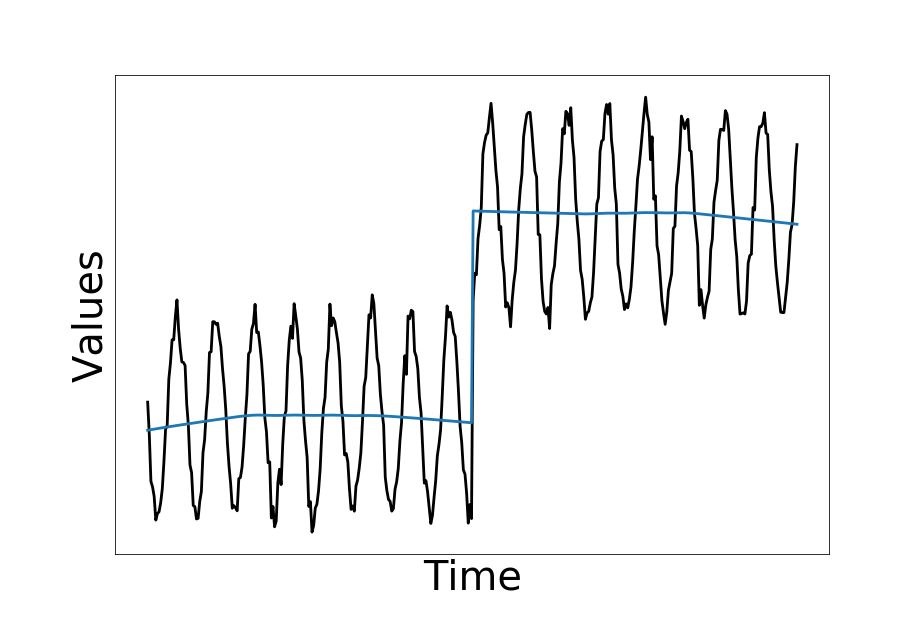
\includegraphics[height=3.5cm]{images/trend_succeed}
	\end{figure}
        \end{column}
    \end{columns}

What can we do after change point detection:
    \begin{itemize}
    	\item Remove/change outliers
	\item Split time series and analyze separately
    \end{itemize}

\end{frame}


\begin{frame}
    \frametitle{Types of change points}

\begin{columns}
 \begin{column}{0.5\textwidth}

  \begin{columns}
      \begin{column}{0.3\textwidth}
      \centering
      Trend change
      \end{column}
      \begin{column}{0.5\textwidth}
      \begin{figure}
		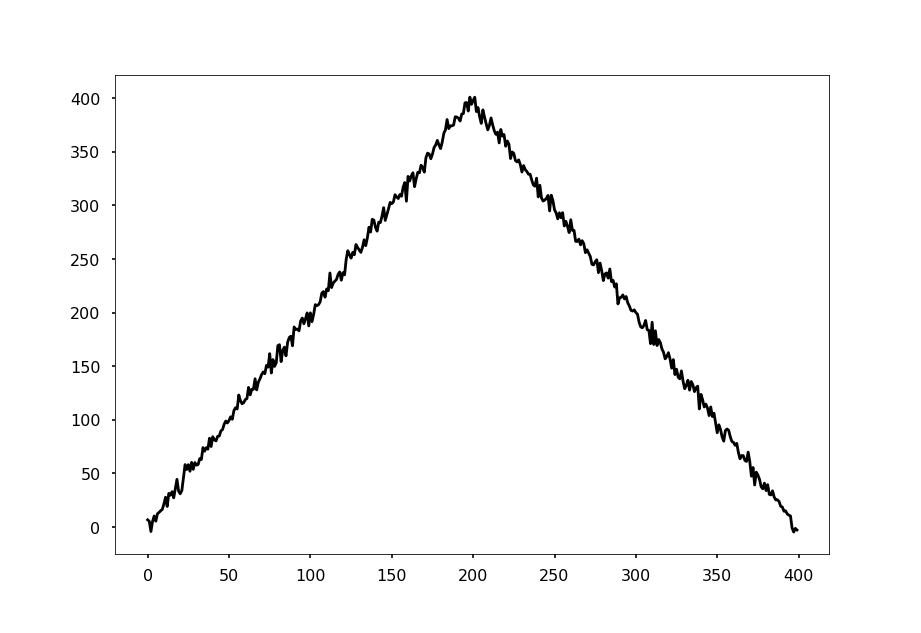
\includegraphics[scale=0.08]{images/examples_trend}
	\end{figure}
	\end{column}
     \end{columns}

  \begin{columns}
      \begin{column}{0.3\textwidth}
      \centering
      Mean change
      \end{column}
      \begin{column}{0.5\textwidth}
      \begin{figure}
		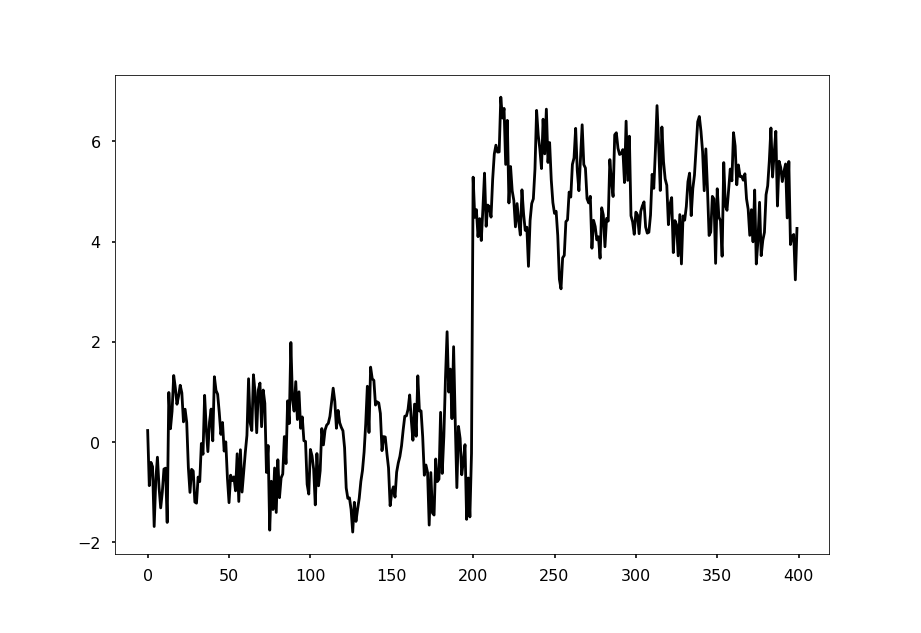
\includegraphics[scale=0.08]{images/examples_mean}
	\end{figure}
	\end{column}
     \end{columns}

  \begin{columns}
      \begin{column}{0.3\textwidth}
      \centering
      Variance change
      \end{column}
      \begin{column}{0.5\textwidth}
      \begin{figure}
		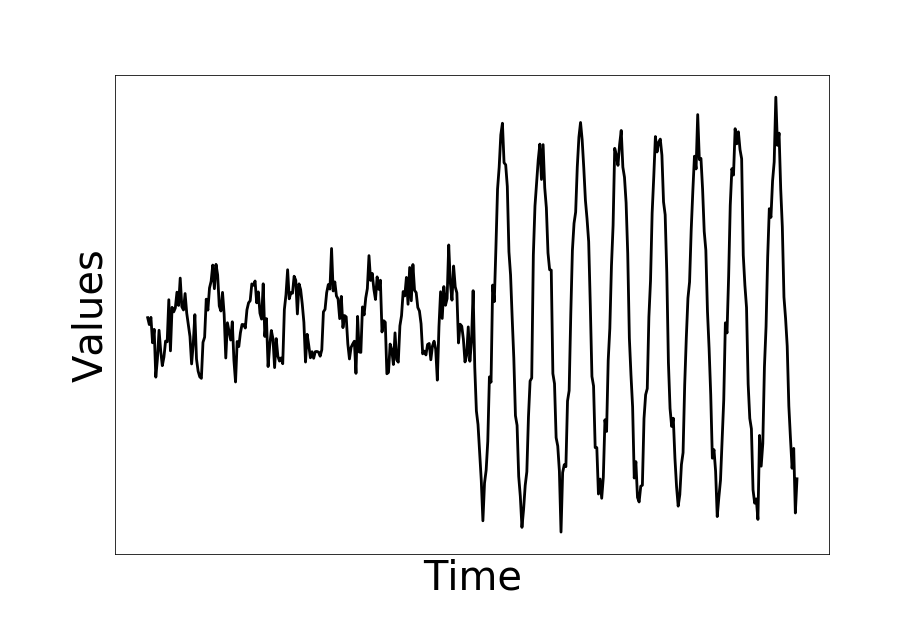
\includegraphics[scale=0.08]{images/examples_variance}
	\end{figure}
	\end{column}
     \end{columns}

	\end{column}

 \begin{column}{0.5\textwidth}

  \begin{columns}
      \begin{column}{0.3\textwidth}
      \centering
      Local change
      \end{column}
      \begin{column}{0.5\textwidth}
      \begin{figure}
		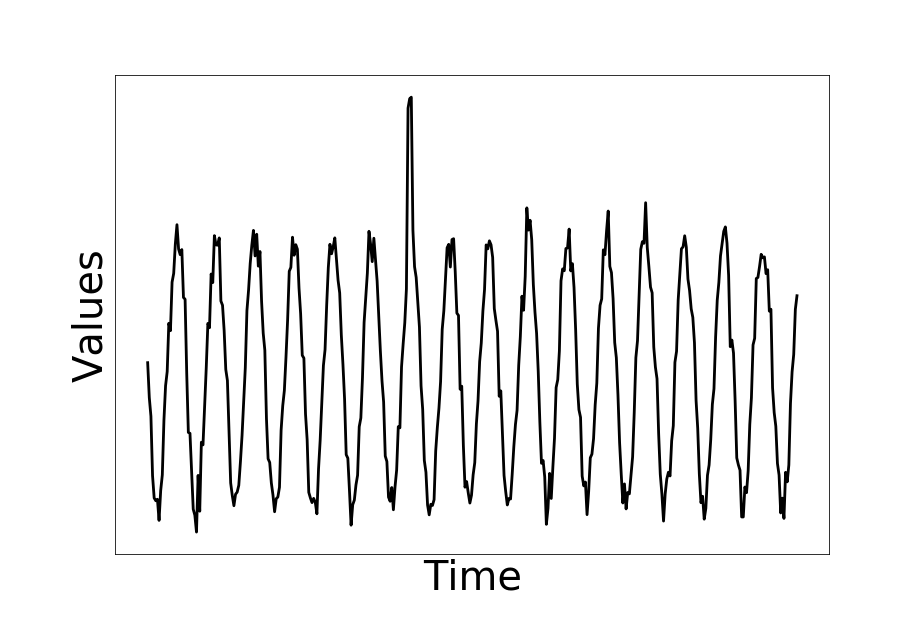
\includegraphics[scale=0.08]{images/examples_outlier}
	\end{figure}
	\end{column}
     \end{columns}

  \begin{columns}
      \begin{column}{0.3\textwidth}
      \centering
      Periodic component change
      \end{column}
      \begin{column}{0.5\textwidth}
      \begin{figure}
		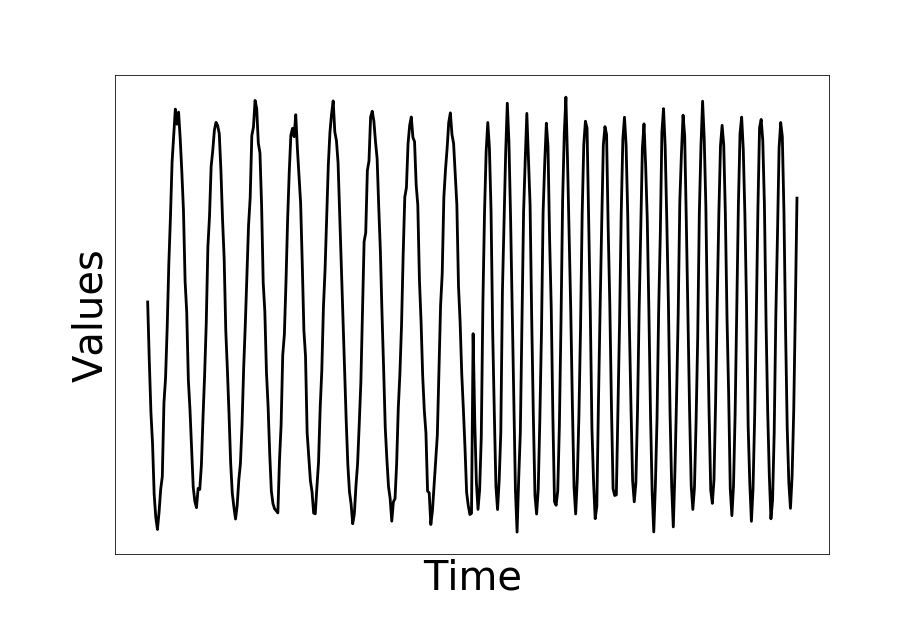
\includegraphics[scale=0.08]{images/examples_periodic}
	\end{figure}
	\end{column}
     \end{columns}

	\end{column}
	
     \end{columns}

\end{frame}


\section{Mobile advertising data}


\begin{frame}
\frametitle{Real data description}

   \begin{columns}
    \begin{column}{0.25\textwidth}
    \centering
     Request
     \begin{figure}
	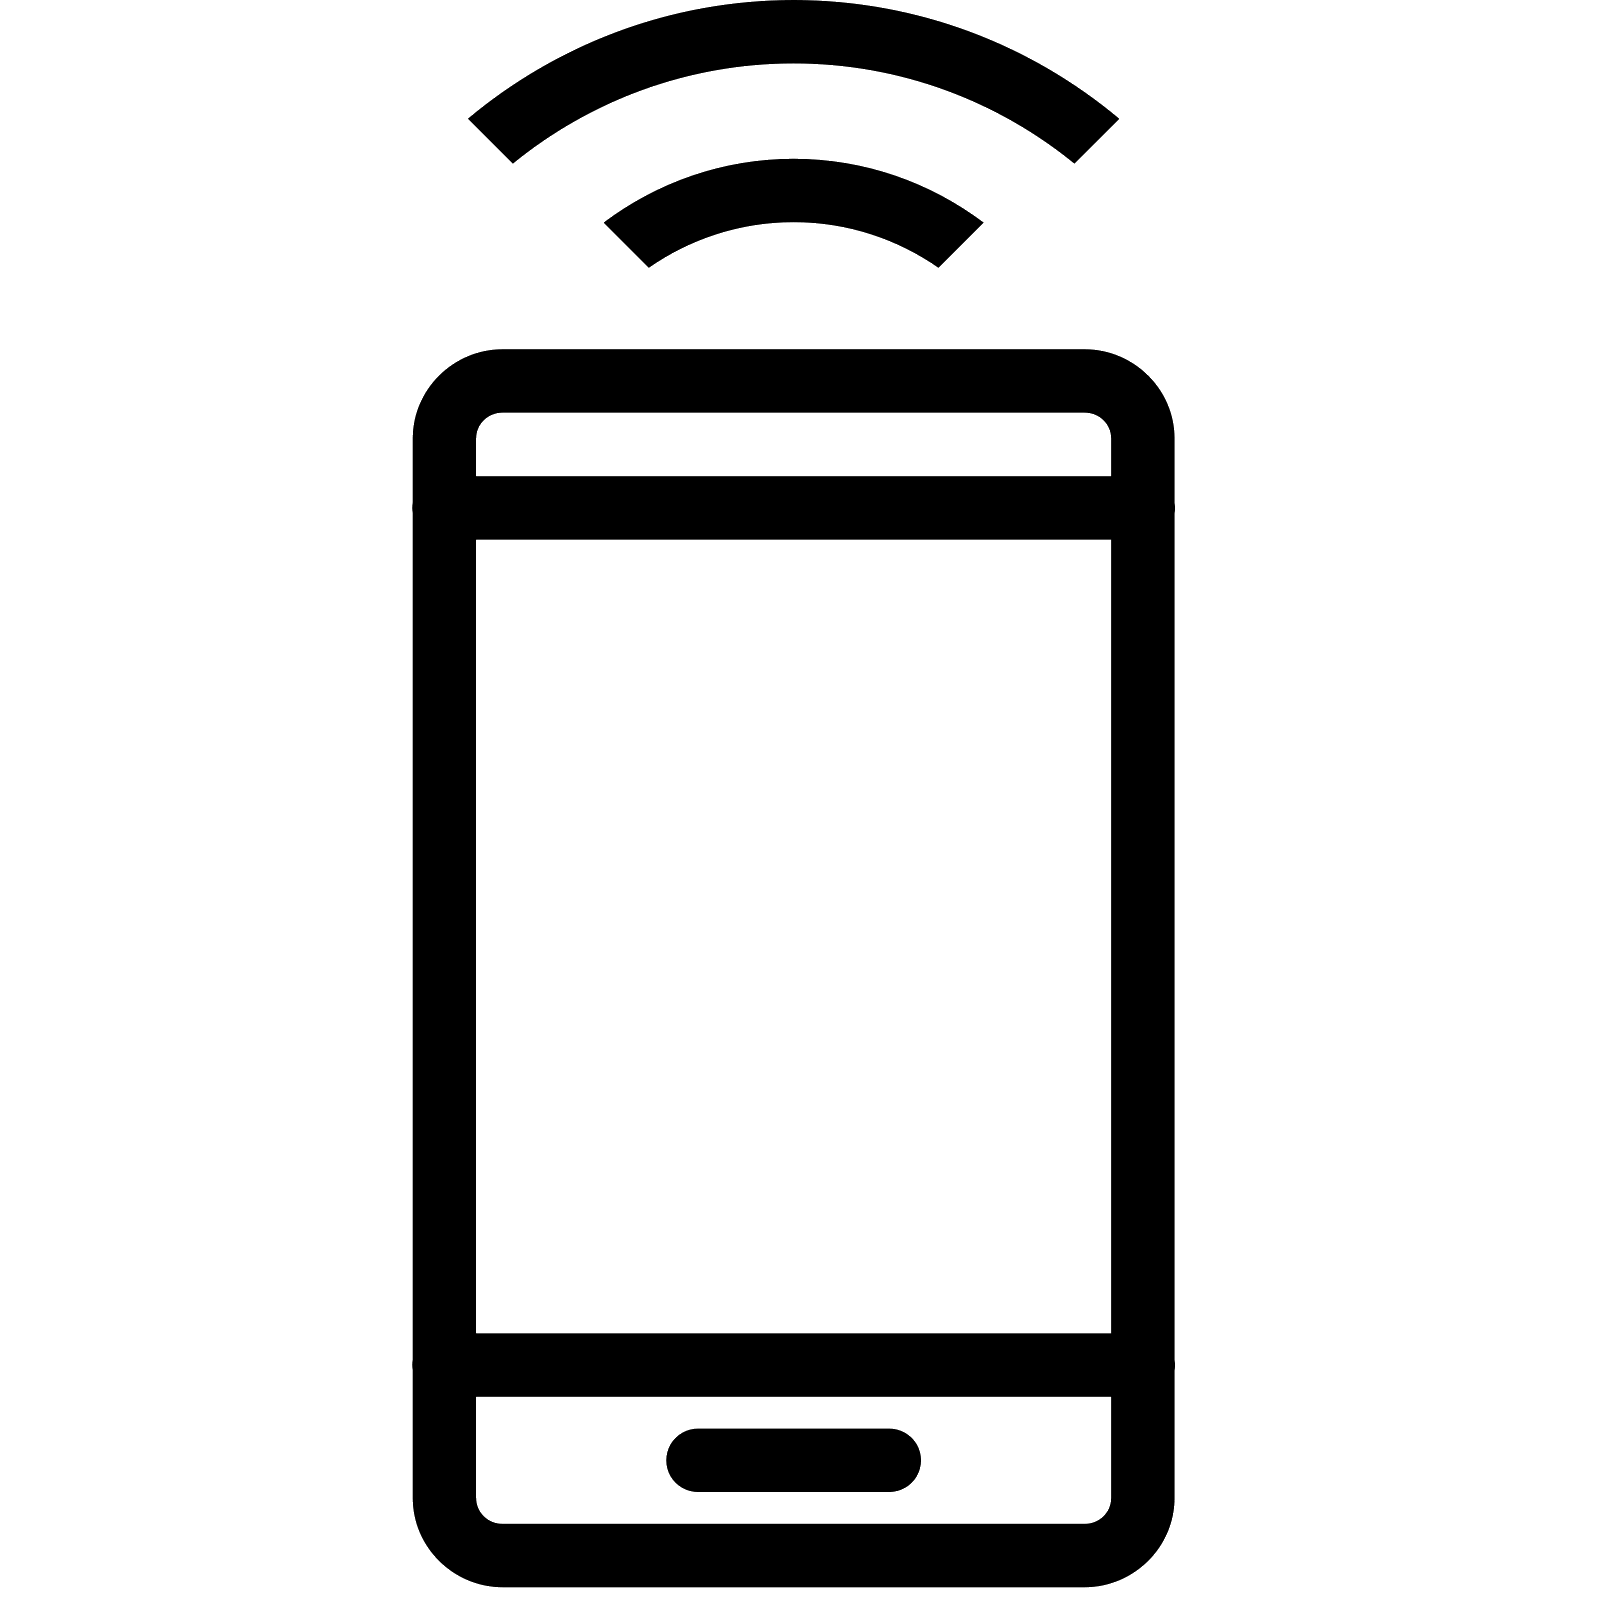
\includegraphics[height=1cm]{images/scheme_request}
     \end{figure}
     \end{column}
    \begin{column}{0.001\textwidth}
    \centering
	>
     \end{column}
    \begin{column}{0.25\textwidth}
    \centering
    Impression
     \begin{figure}
	
\includegraphics[height=1cm]{images/scheme_impression}
     \end{figure}
    \end{column}
    \begin{column}{0.001\textwidth}
    \centering
    >
    \end{column}
    \begin{column}{0.25\textwidth}
    \centering
    Click
     \begin{figure}
	
\includegraphics[height=1cm]{images/scheme_click}
     \end{figure}
    \end{column}
    \begin{column}{0.001\textwidth}
    \centering
    >
    \end{column}
    \begin{column}{0.25\textwidth}
    \centering
     Conversion
     \begin{figure}
	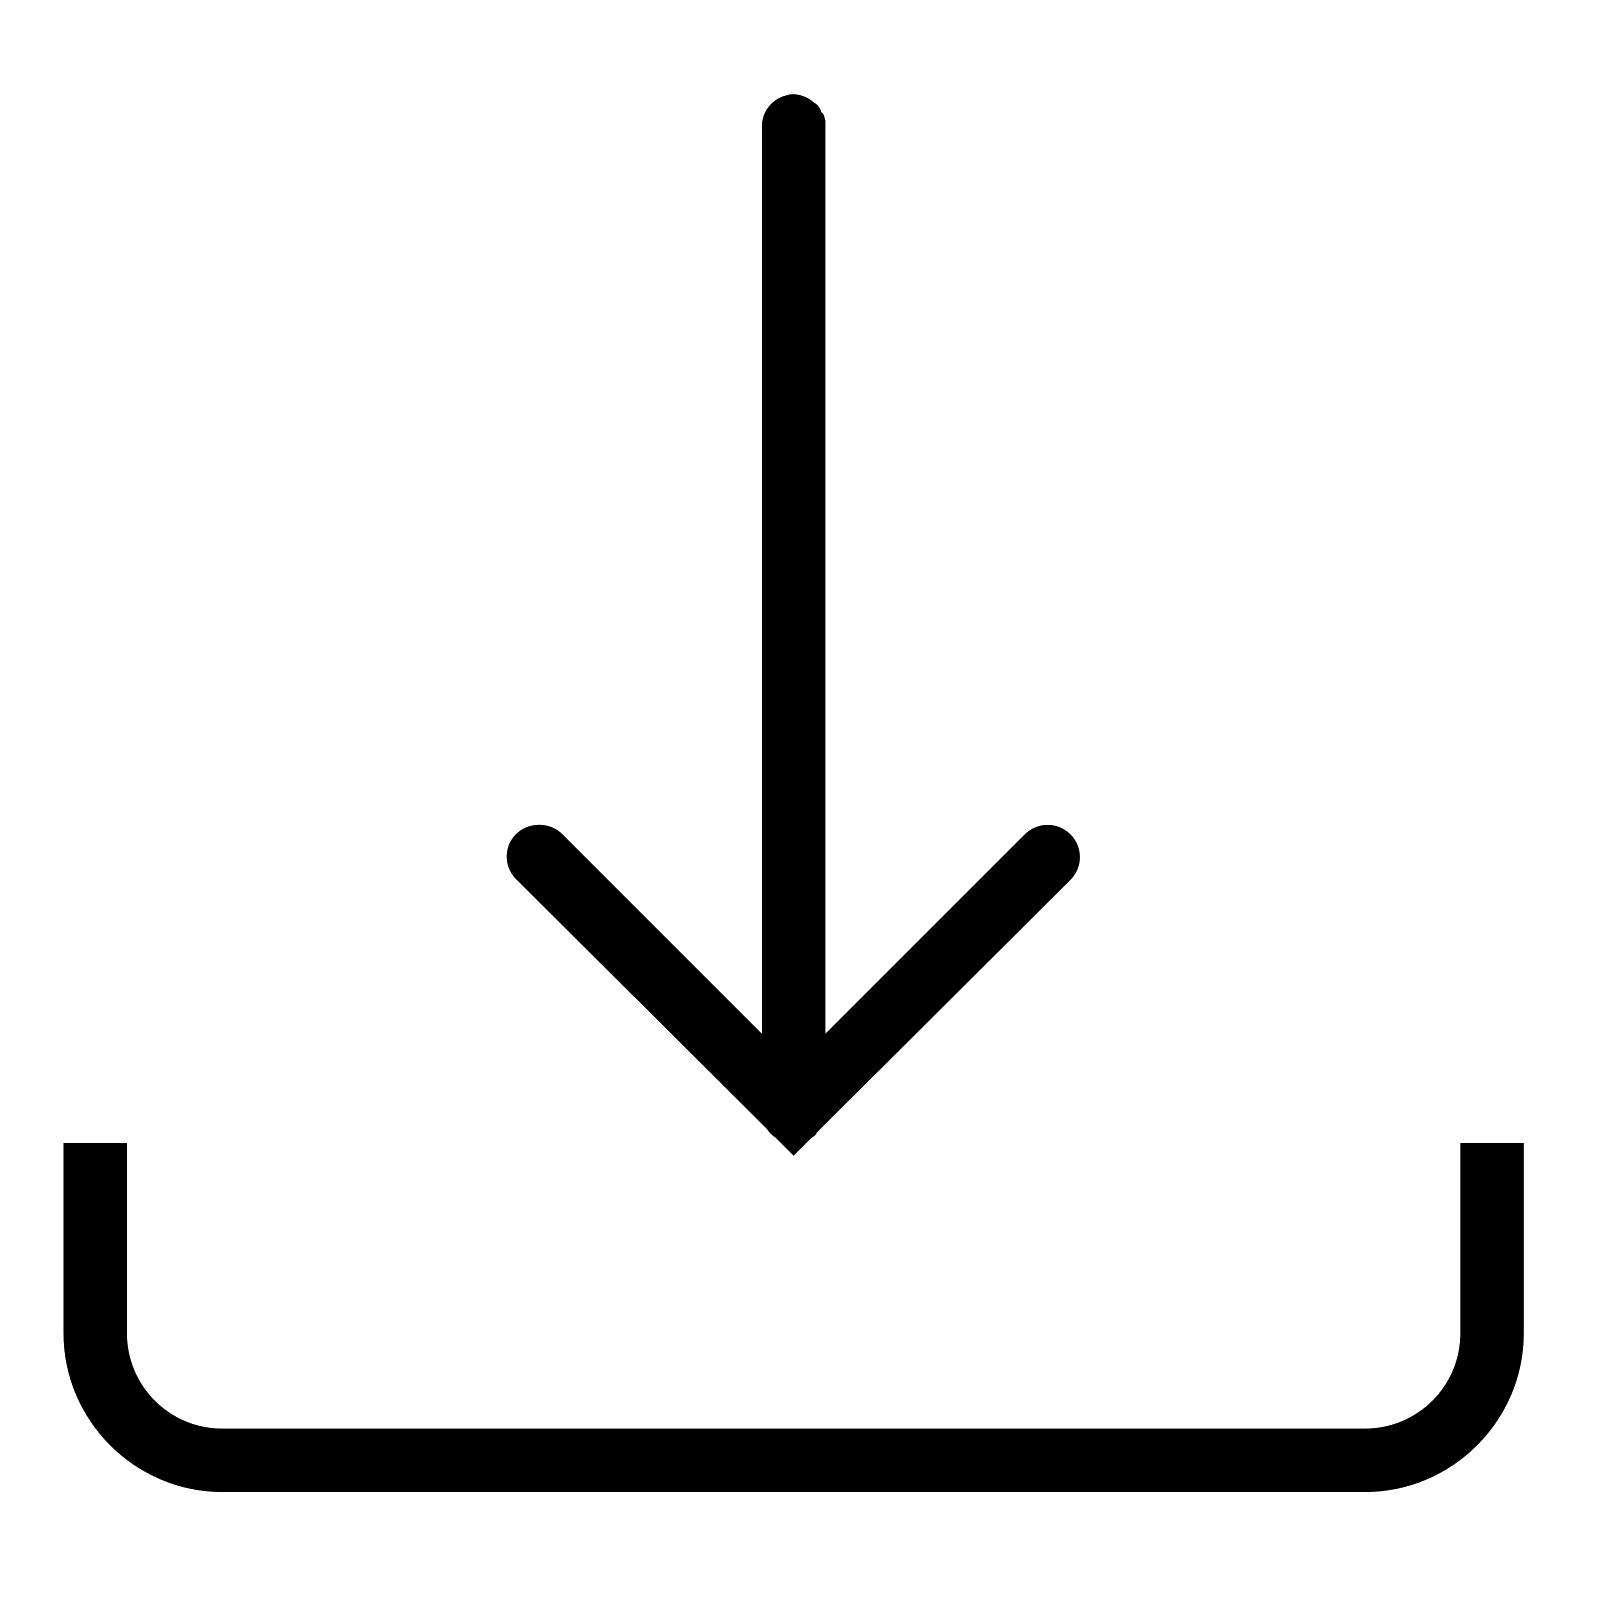
\includegraphics[height=1cm]{images/scheme_conversion}
     \end{figure}
     \end{column}
     \end{columns}

   \begin{columns}
    \begin{column}{0.5\textwidth}
	\begin{figure}
	\textbf{Typical day}\par\medskip
	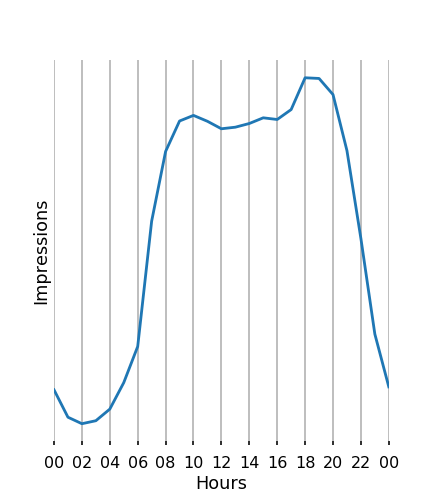
\includegraphics[height=4.5cm]{images/examples_day}
	\end{figure}
     \end{column}
    \begin{column}{0.5\textwidth}
	\begin{figure}
	\textbf{Typical weekend}\par\medskip
	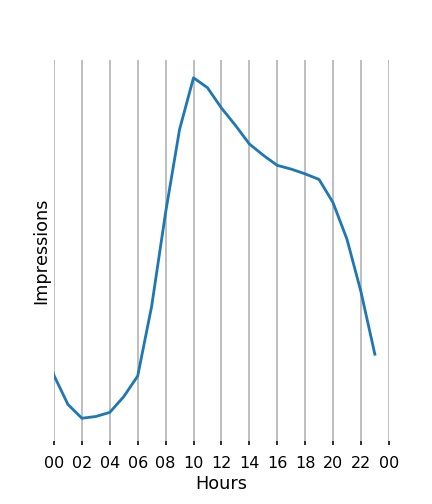
\includegraphics[height=4.5cm]{images/examples_weekend}
	\end{figure}
     \end{column}
     \end{columns}

\end{frame}

\begin{frame}
\frametitle{Real data example}
\begin{figure}
\textbf{Typical hourly impressions}\par\medskip
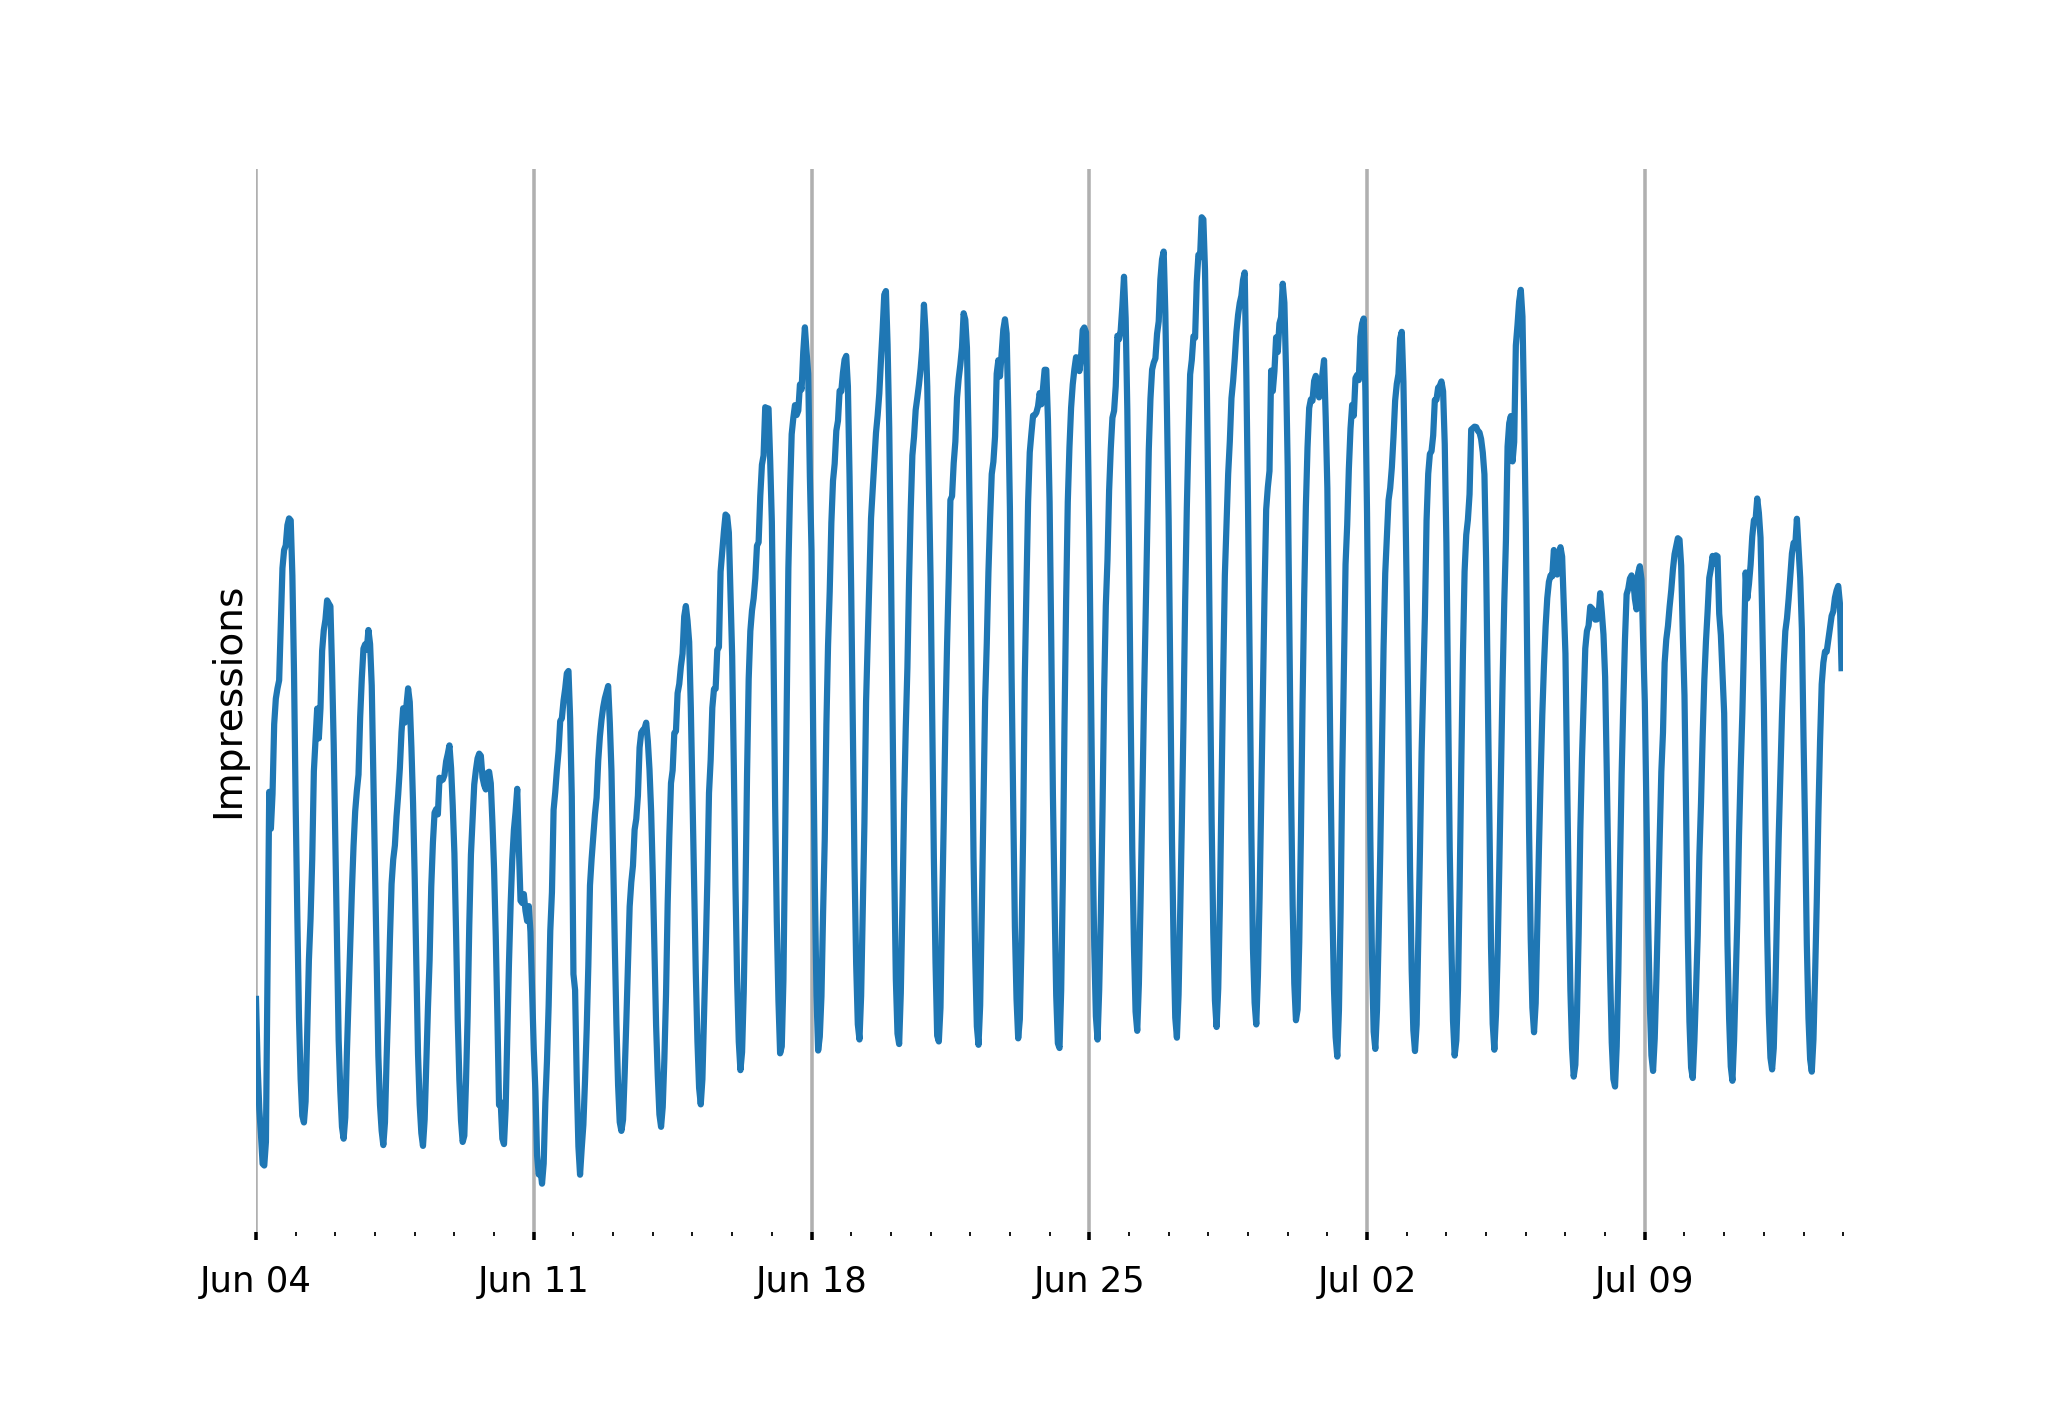
\includegraphics[scale=0.30]{images/examples_month}
\end{figure}
\end{frame}

\begin{frame}
\frametitle{Real data example}
\begin{figure}
\textbf{Typical hourly impressions}\par\medskip
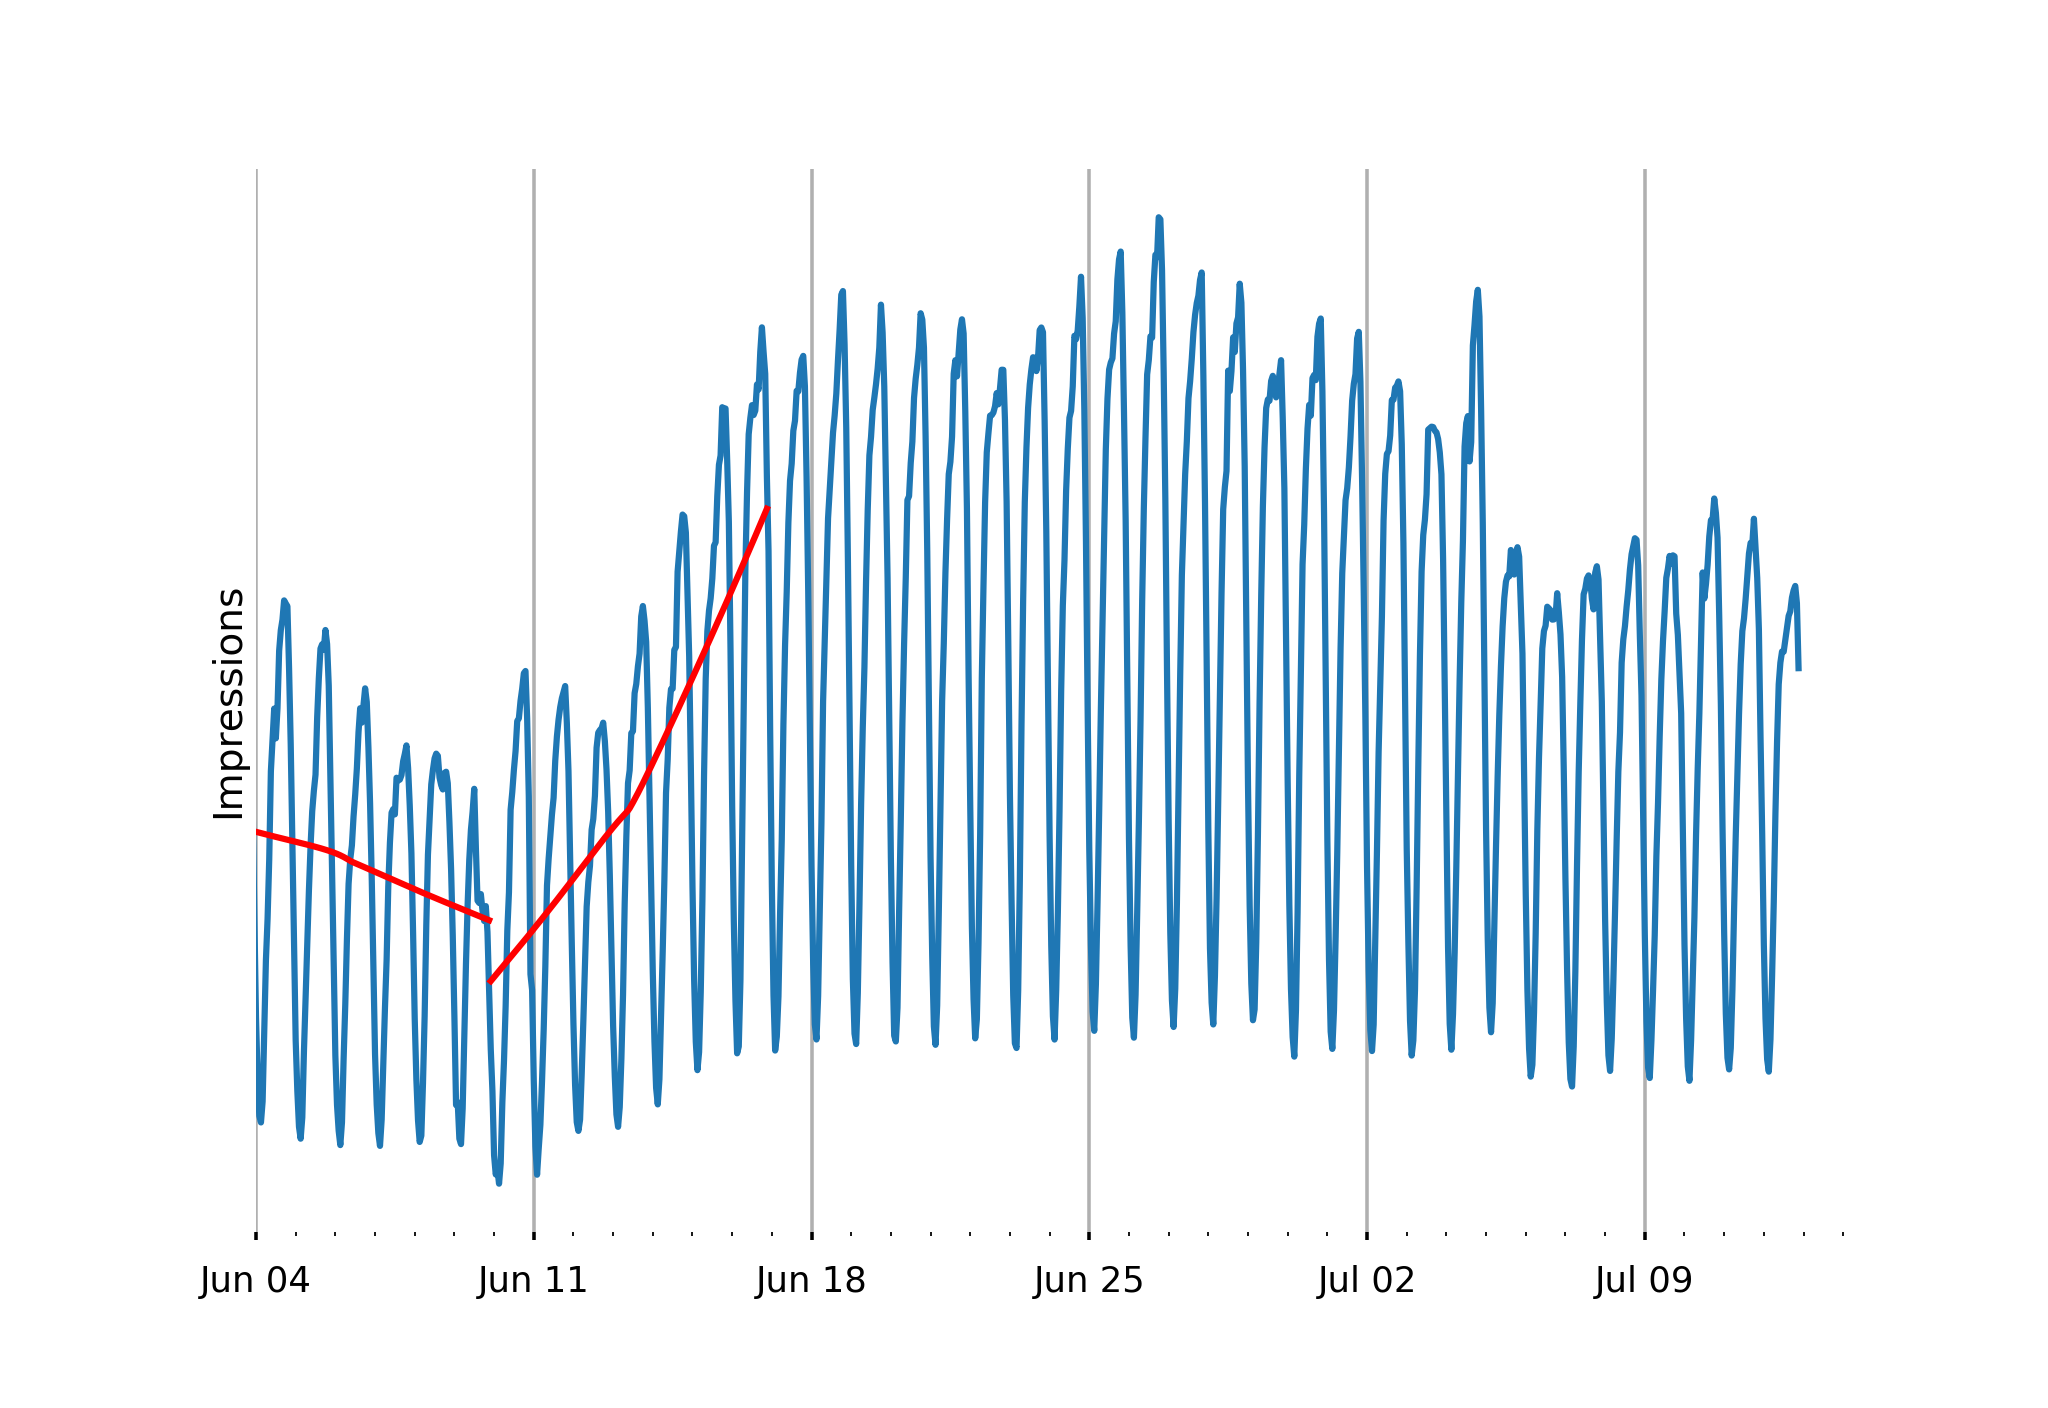
\includegraphics[scale=0.30]{images/examples_month_2}
\end{figure}
\end{frame}

\begin{frame}
\frametitle{Real data example}
\begin{figure}
\textbf{Typical hourly impressions}\par\medskip
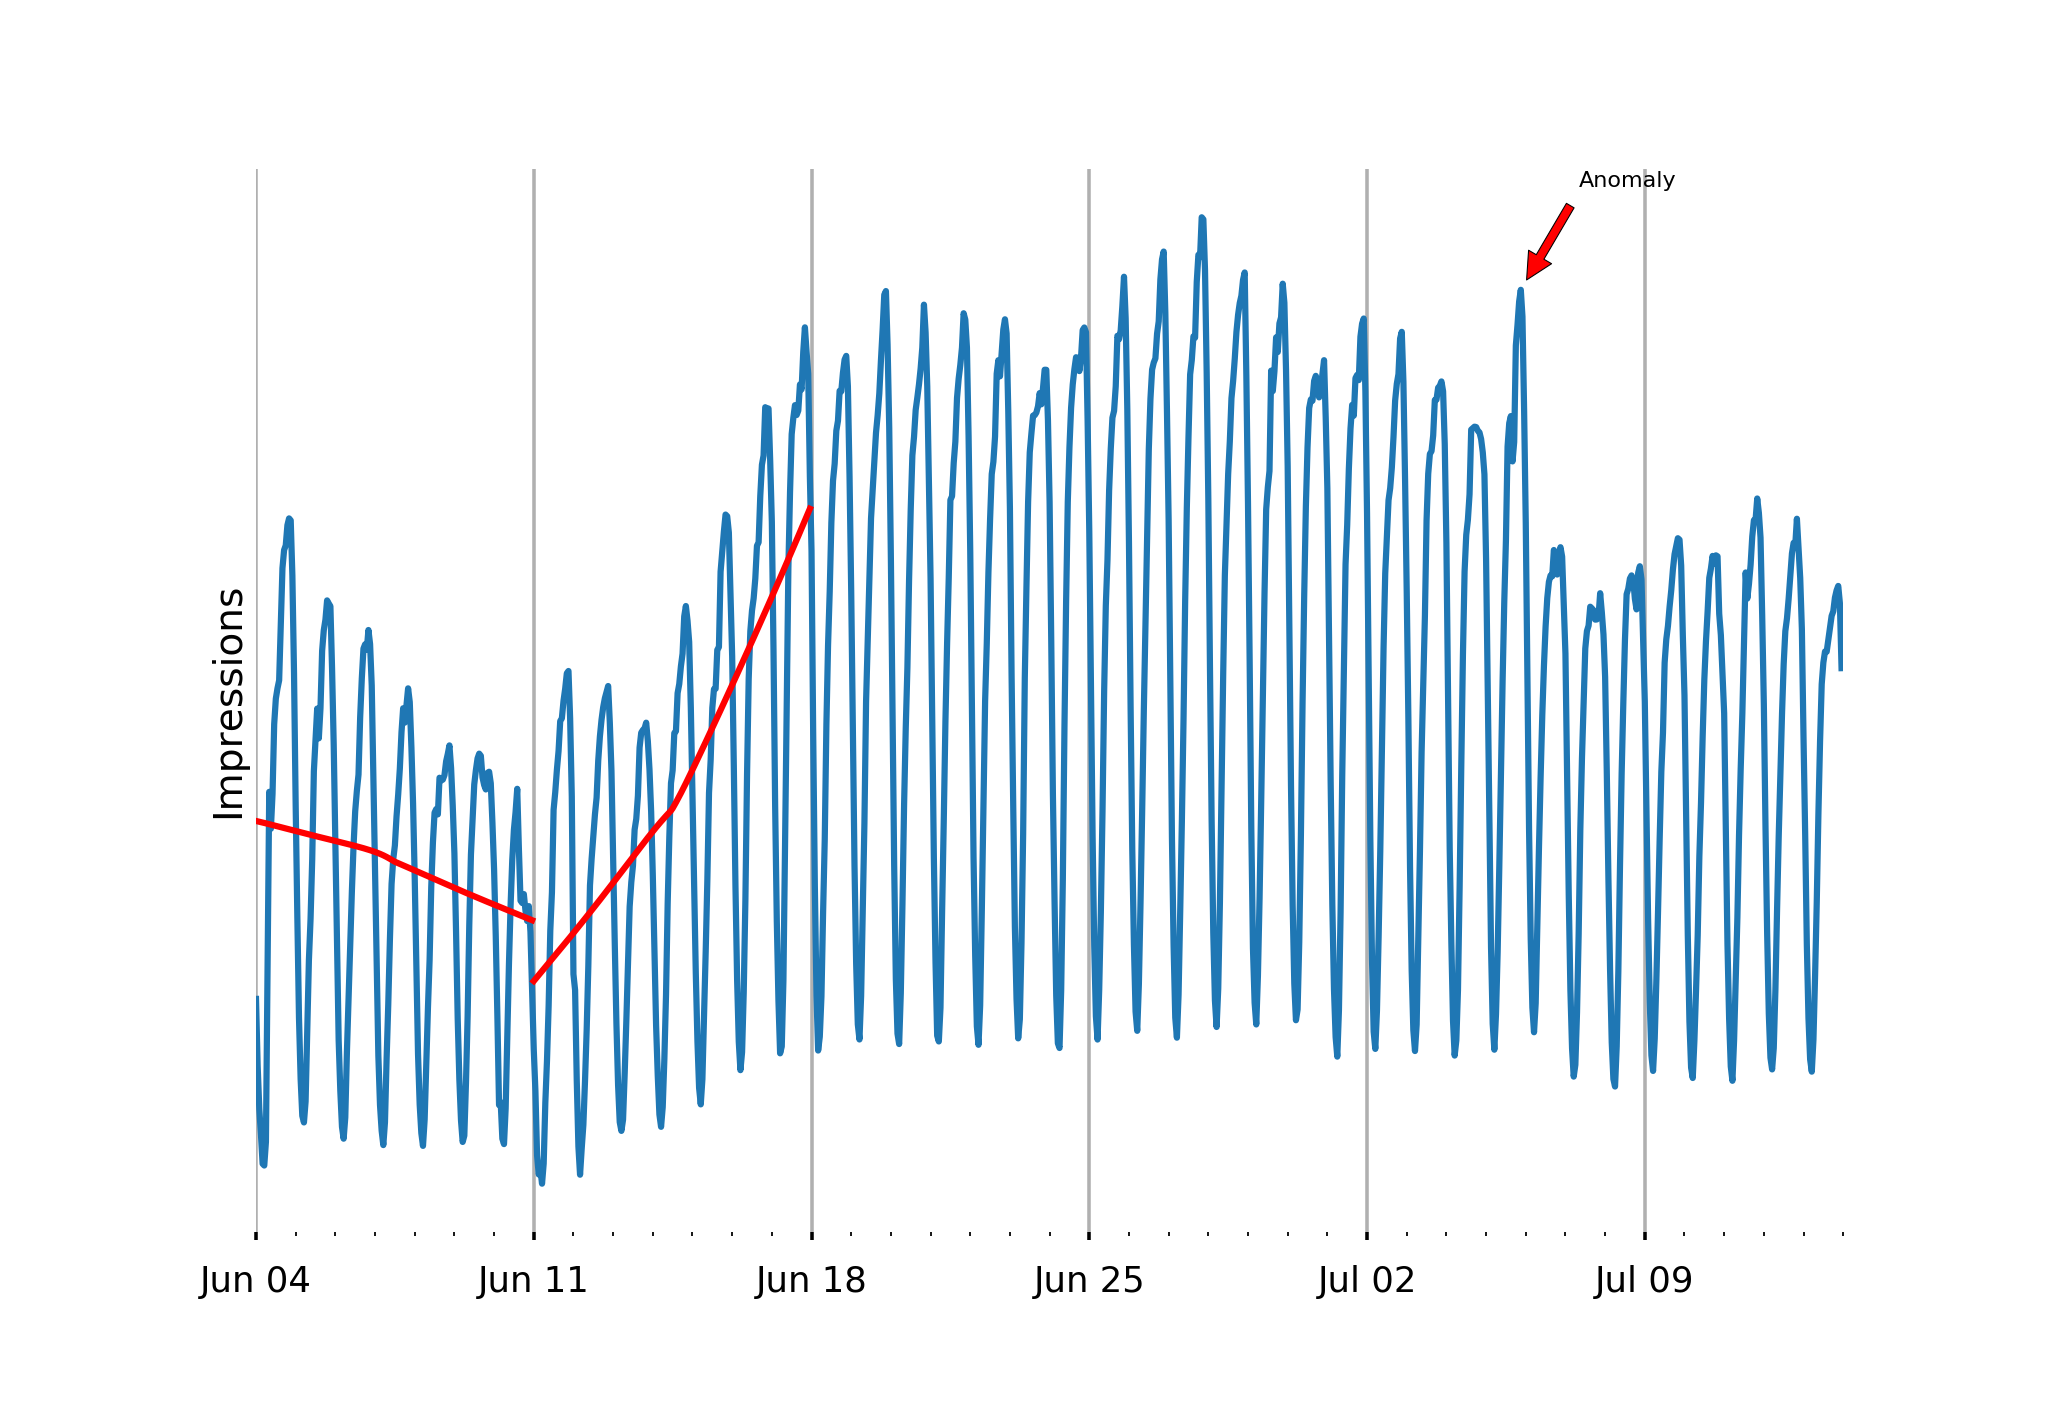
\includegraphics[scale=0.30]{images/examples_month_3}
\end{figure}
\end{frame}

\begin{frame}
\frametitle{Change point examples}
\begin{figure}
\textbf{Mean change}\par\medskip
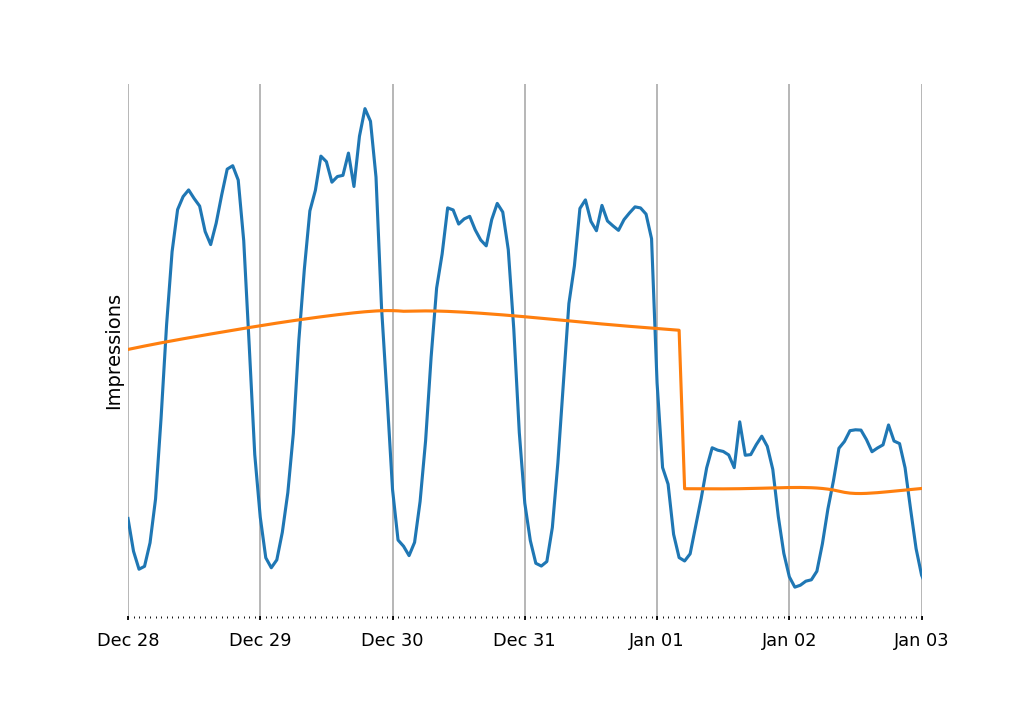
\includegraphics[scale=0.30]{images/1_examples_mean}
\end{figure}
\end{frame}


\begin{frame}
\frametitle{Change point examples}
\begin{figure}
\textbf{Local change (outlier)}\par\medskip
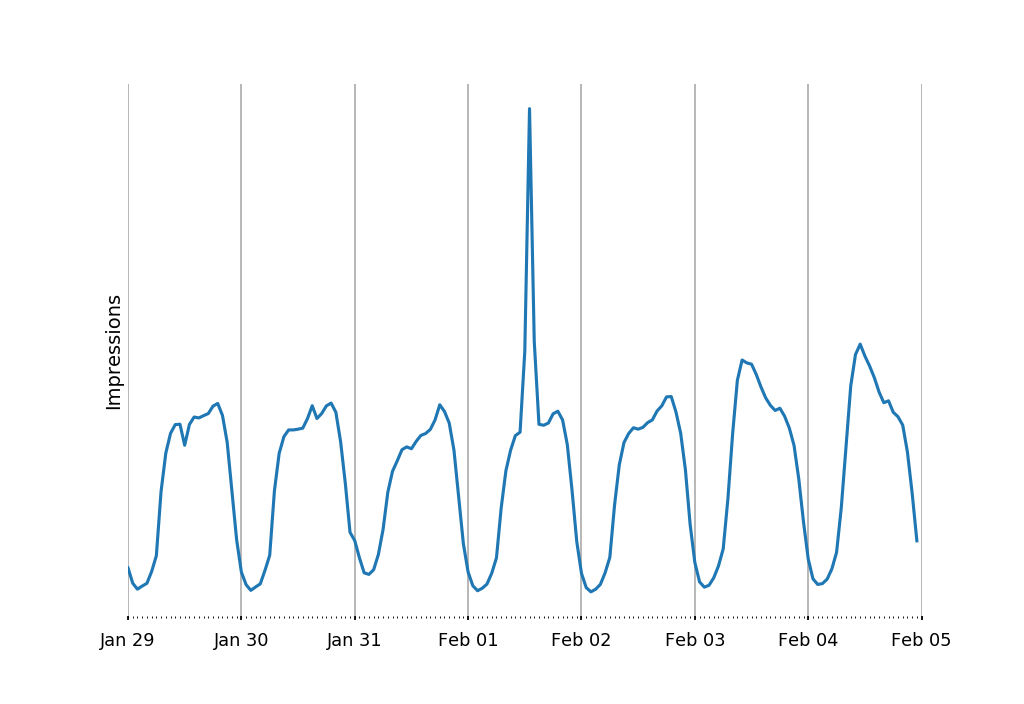
\includegraphics[scale=0.30]{images/005_point}
\end{figure}
\end{frame}

\begin{frame}
\frametitle{Change point examples}
\begin{figure}
\textbf{Periodic component change}\par\medskip
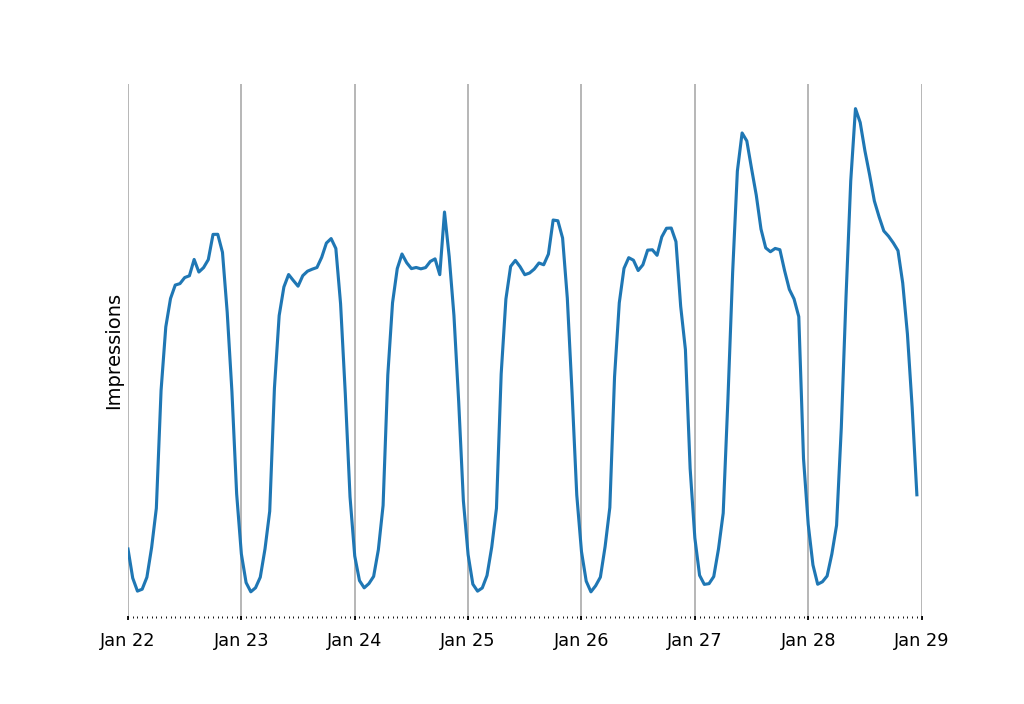
\includegraphics[scale=0.30]{images/006_structure}
\end{figure}
\end{frame}


\section{Change point detection techniques}


%\begin{frame}
  %  \frametitle{Methods}



%  \begin{columns}[T,onlytextwidth]
  %    \column{0.5\textwidth}
    %  Naïve approach
    %\begin{itemize}
    %	\item Calculate \% difference with previous period
%	\item Compare difference with threshold
  %  \end{itemize}

%     \end{columns}

%\end{frame}

% \begin{frame}
%    \frametitle{General framework description}
%
% 	    \begin{itemize}
% 		\item Algorithm:
% 		\begin{itemize}
% 			\item Cost value is calculated for sliding windows of time series
% 			\item Cost value represents how different our model from actual data
% 			\item Once cost value more than threshold - algorithm detects change point
% 		\end{itemize}
% 		\item Types:
% 		\begin{itemize}
% 			\item Prediction based
% 			\item Approximation based
% 		\end{itemize}
% 	    	\item Input:
% 		\begin{itemize}
% 			\item Window size
% 			\item Model
% 			\item Cost function
% 			\item Threshold
% 			\item Search method
% 		\end{itemize}
% 	    \end{itemize}

% \end{frame}


\begin{frame}
    \frametitle{General framework description}

	    \begin{itemize}
		\item \textblue{Preliminaries}:
		\begin{itemize}
			\item Time series has a structure\\ (e.g. a constant trend)
\vspace{0.1cm}
			\item Structure can be described by a model\\
             (e.g. the time series is equal to sum of a constant and some oscillations)
\vspace{0.1cm}
            \item Structure is abruptly changed; we should detect this change
\vspace{0.1cm}
            \item Types of changes are different; therefore, we need different methods to detect
		\end{itemize}

\vspace{0.2cm}
		\item \textblue{Approach}:
		\begin{itemize}
			\item Around the change point (CP), model describes time series worse
			\item We can calculate this ``worseness'' using cost function
			\item Once cost value more than threshold - algorithm detects change point
		\end{itemize}

\vspace{0.2cm}
		\item \textblue{Types of methods}:
		\begin{itemize}
			\item Prediction based
			\item Approximation based
		\end{itemize}
	    \end{itemize}

\end{frame}



\begin{frame}
    \frametitle{Prediction approach}

  \begin{columns}[T,onlytextwidth]
      \column{0.5\textwidth}
	\textbf{Prediction based approach}
	    \begin{itemize}
	    \onslide<1,2->{\item Predict with appropriate model}
		\onslide<1,3->{\item Measure difference between prediction and actual data}
		\onslide<1,4->{\item Perform this for sliding subseries (windows)}
 		\onslide<1,5->{\item Construct detection function with difference measures}
 		\onslide<1,5->{\item Compare with threshold}
	    \end{itemize}
      \column{0.5\textwidth}
      Example: change in mean; model is a constant trend
      \begin{figure}
	\only<1>{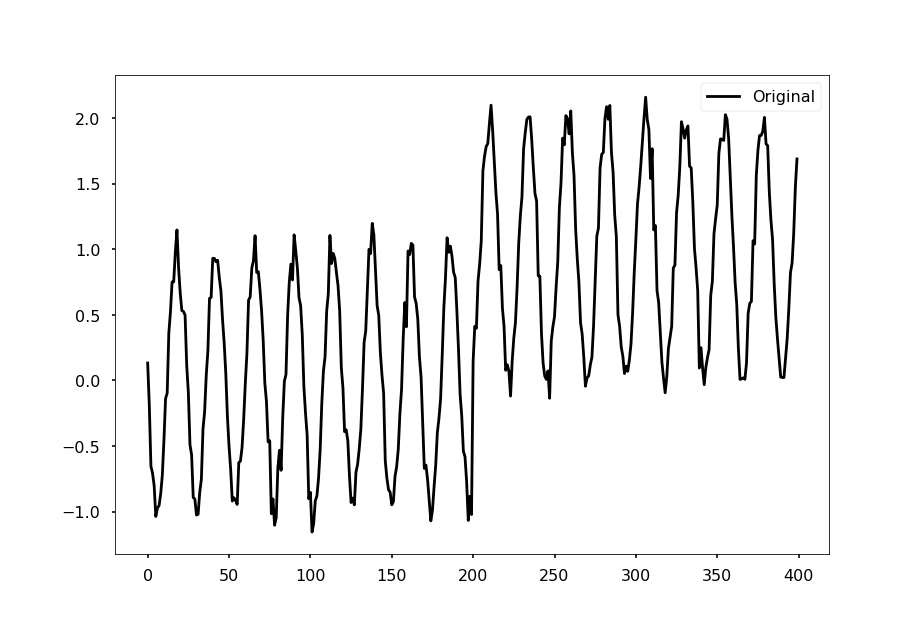
\includegraphics[scale=0.2]{images/approaches_first_1}}
	\only<2>{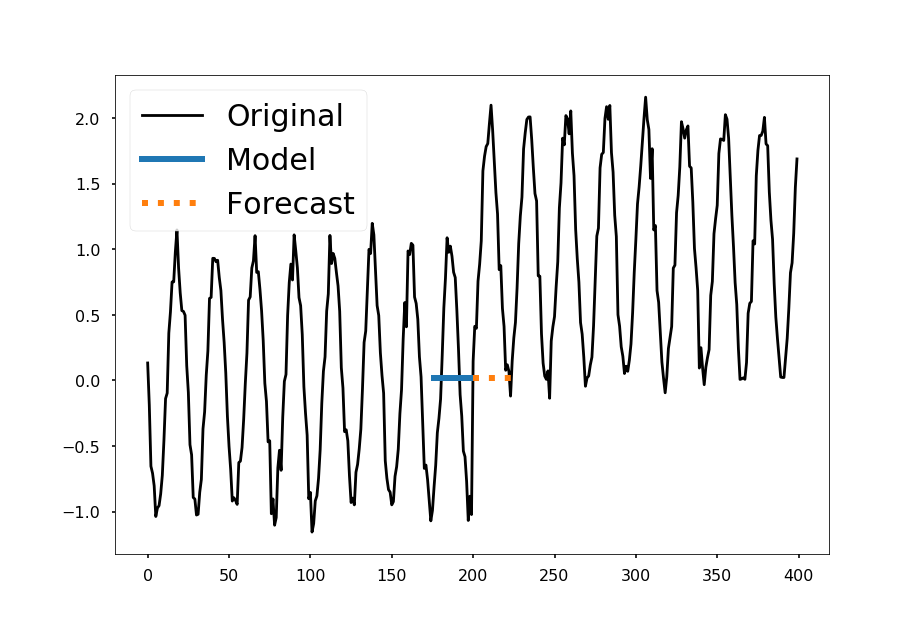
\includegraphics[scale=0.2]{images/approaches_first_3}}
	\only<3>{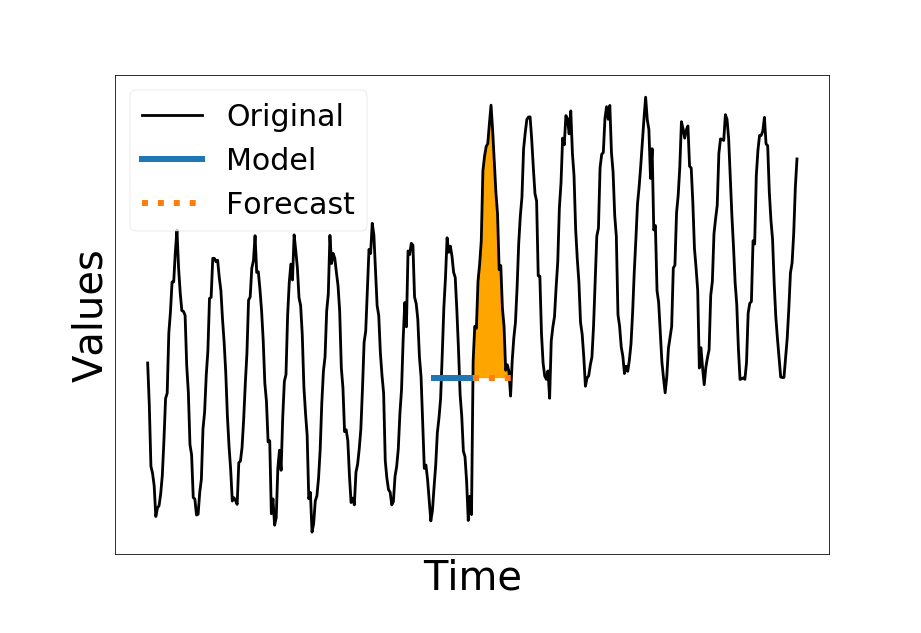
\includegraphics[scale=0.2]{images/approaches_first_4}}
	\only<4,5>{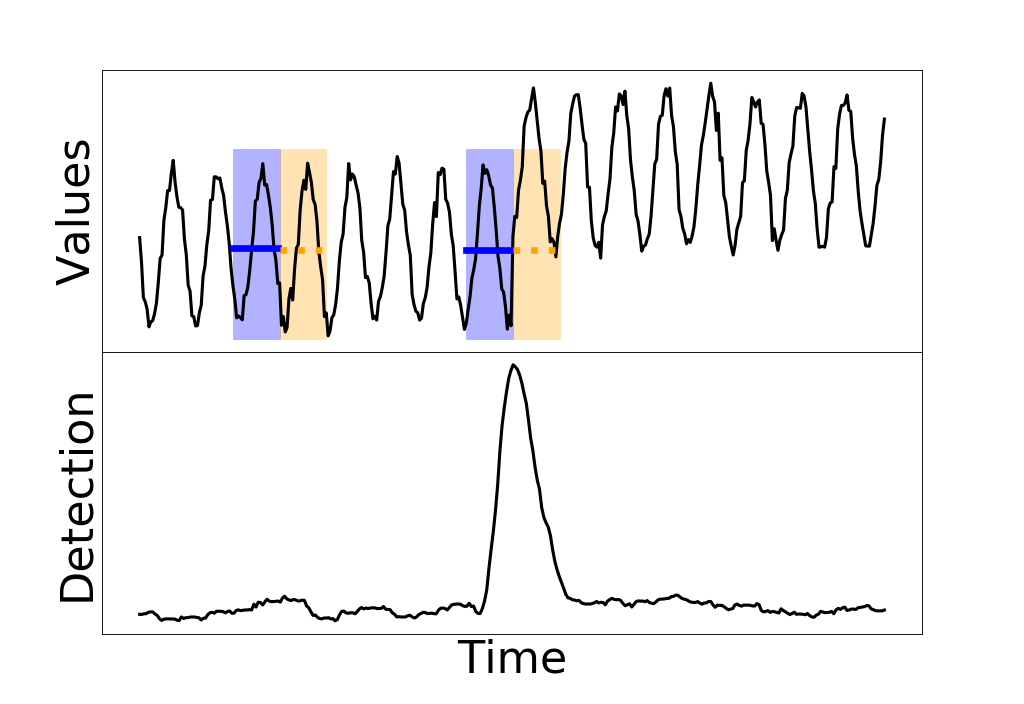
\includegraphics[scale=0.2]{images/approaches_first_5}}
	\only<5>{Detection function is synchronized with the last point of window}
	\end{figure}
     \end{columns}

\end{frame}

\begin{frame}
    \frametitle{Approximation approach}

  \begin{columns}[T,onlytextwidth]
      \column{0.5\textwidth}
	\textbf{Approximation based approach}
	    \begin{itemize}
	    \onslide<1->{\item Approximate time series with appropriate model}
		\item 
        \onslide<2->{\only<2>{Measure difference between \textblue{approximation errors for left and right halves separately}}
        \only<1,3->{Measure difference between approximation errors for left and right halves separately}}
        \onslide<3->{\only<3>{and \textblue{the overall approximation error}}
        \only<1,2,4->{and the overall approximation error}}
		\onslide<4->{\item Perform this for sliding subseries (windows)}
 		\onslide<5->{\item Construct detection function with difference measures}
 		\onslide<5->{\item Compare with threshold}
	    \end{itemize}
      \column{0.5\textwidth}
      Example: change in mean; model is a constant trend
      \begin{figure}
	\only<1>{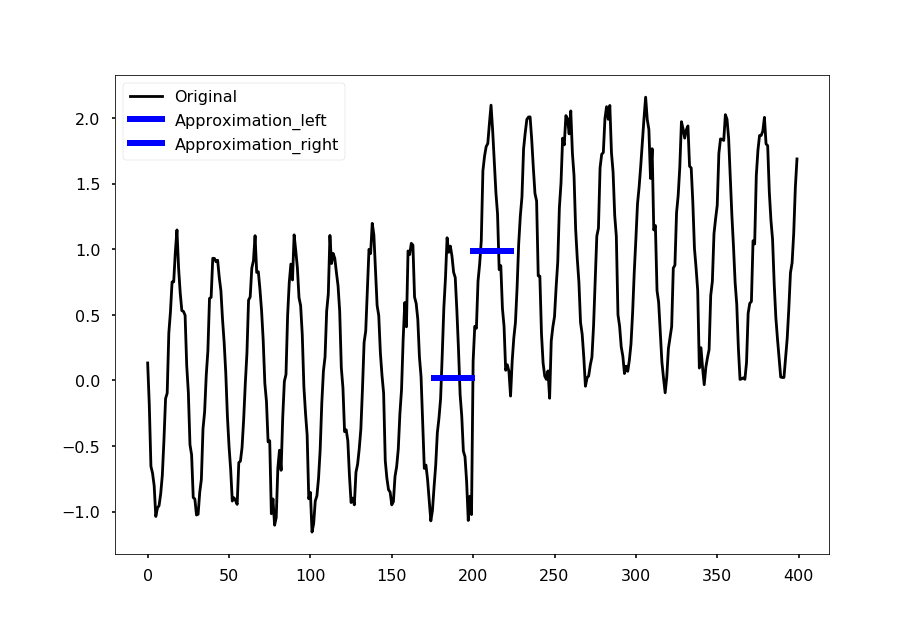
\includegraphics[scale=0.2]{images/approaches_second_1}}
	\only<2>{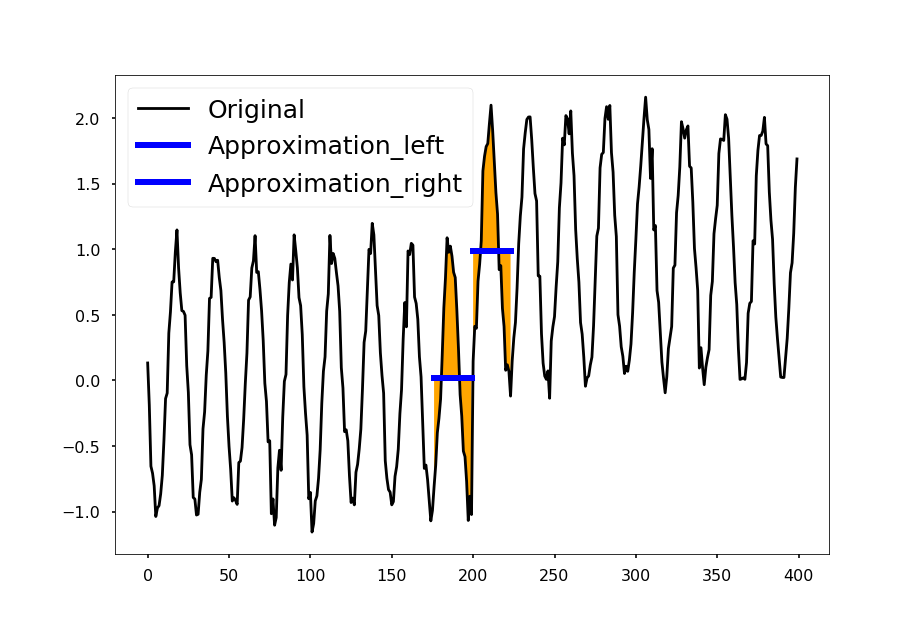
\includegraphics[scale=0.2]{images/approaches_second_2}}
	\only<3>{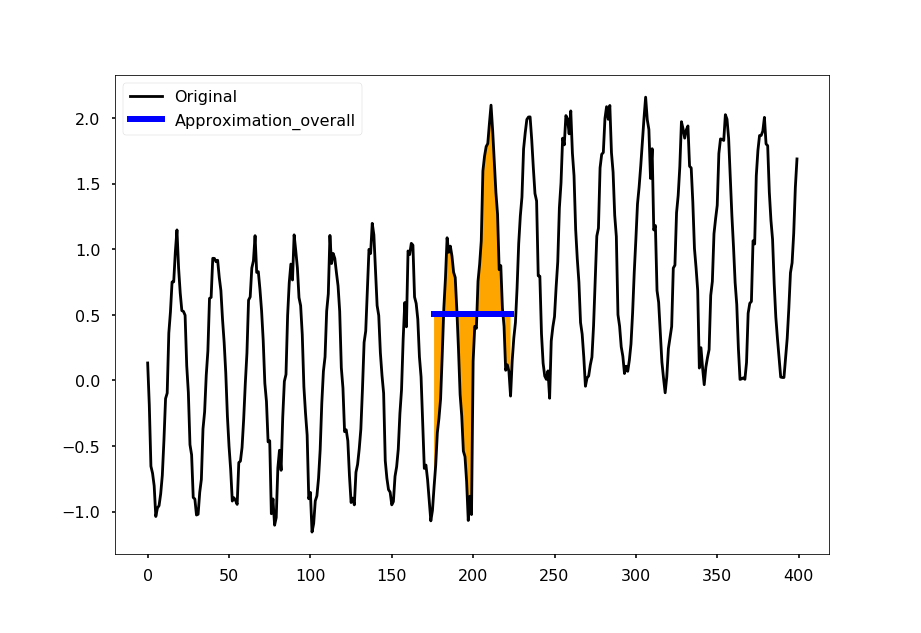
\includegraphics[scale=0.2]{images/approaches_second_3}}
	\only<4,5>{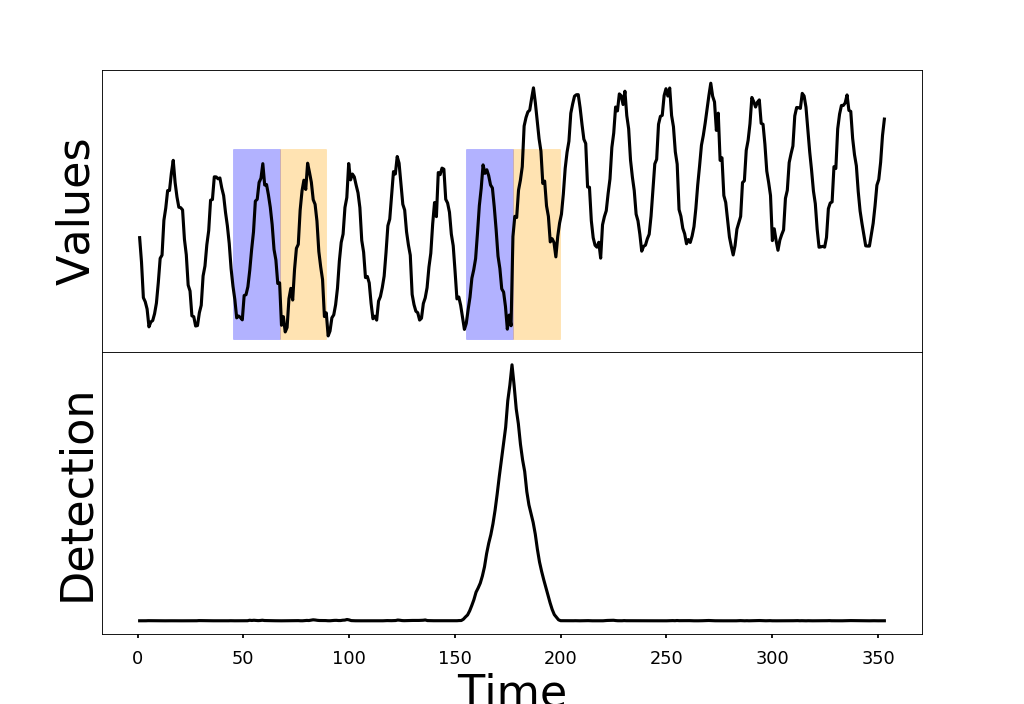
\includegraphics[scale=0.2]{images/approaches_second_4}}
	\only<5>{Detection function is synchronized with the last point of window}
	\end{figure}
     \end{columns}

\end{frame}


\begin{frame}
    \frametitle{Things to define}
	
	\begin{itemize}
	    	\item \textblue{Model}. Based on what changes do you want to find and specifics of your time series
			\begin{itemize}
			\item Data has a constant trend, we are interested in changes in trend (formal model: in the time (e.g., a hour) with number $n$, $x_n = \mathrm{const} + \mathrm{residual}_n$).
\smallskip
			\item Data has a linear trend, we are interested in changes in trend (formal model: $x_n = an+b + \mathrm{residual}_n$).
\smallskip
			\item Data has a constant trend with regular (e.g. daily) fluctuations, we are interested in changes in trend or in fluctuations (formal model: $x_n = \mathrm{const} + A\sin(2\pi n/24+\phi) + \mathrm{residual}_n$)
\smallskip			
            \item Others
			\end{itemize}
\medskip
		\item \textblue{Window size}. Based on timeframe that is significant to your task. Larger window causes larger delay of detection.
%		\item Cost function. Based on what changes do you want to find.
\medskip
		\item \textblue{Threshold}. Depends on small or big changes would you like to find.
	    \end{itemize}

\bigskip
		Direction of change point search (forward, backward, both directions) depends on your task.


 \end{frame}

\section{Applications to real data}



\begin{frame}
    \frametitle{Applications to real data}
    
    Consider global changes in constant trend and local anomalies

\medskip    
    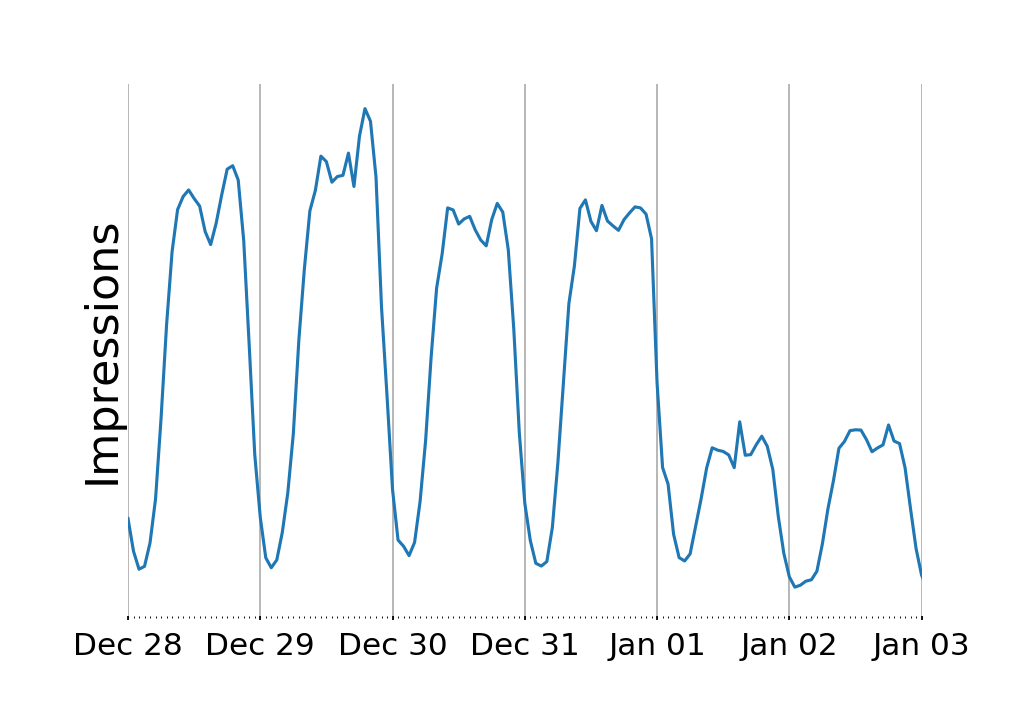
\includegraphics[width = 4cm]{images/cp_mean_2}\qquad
    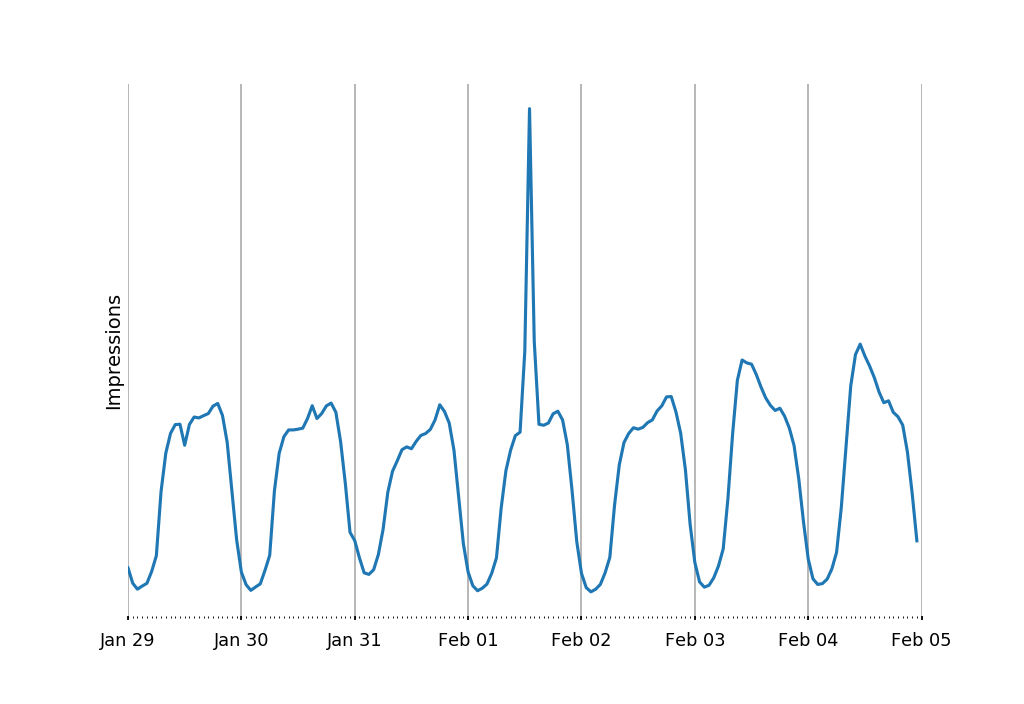
\includegraphics[width = 4cm]{images/005_point}

\medskip
\textblue{Data structure}: constant or slowly varying trend + daily (24-hours) regular oscillations + some noise

\medskip
Two formal \textblue{models}:

\medskip
\begin{enumerate}
\item
Ignore daily oscillations:
$$ x_n = \mathrm{const} + \mathrm{residual}_n $$
\item
Take into consideration daily oscillations:
$$ x_n = \mathrm{const} + A\sin(2\pi n/24+\phi) + \mathrm{residual}_n $$
\end{enumerate}
%Cost function will be mean square error
% $$ c(\mathbf{X}_I) = \sum_{t \in I}||\mathbf{X}_t - \bar{\mathbf{X}} ||_2^2 $$

\medskip
\textblue{Window size} is equal to 2 days; that is, we consider sliding 48-hour subseries.

\medskip
Two \textblue{methods}: prediction- and approximation- based ones.

 \end{frame}



\begin{frame}
    \frametitle{Applications to real data. Mean change}
  \begin{columns}[T,onlytextwidth]
      \column{0.5\textwidth}
	\begin{figure}
	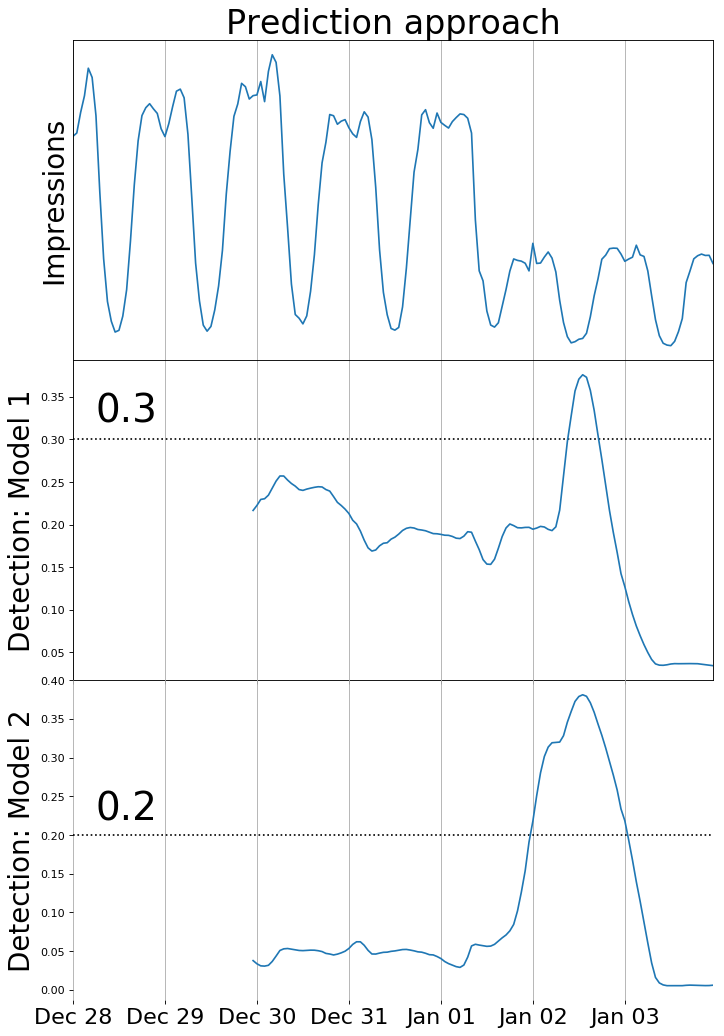
\includegraphics[height=6cm]{images/methods_comparison_1_1}
	\end{figure}
	
      \column{0.5\textwidth}
	\begin{figure}
	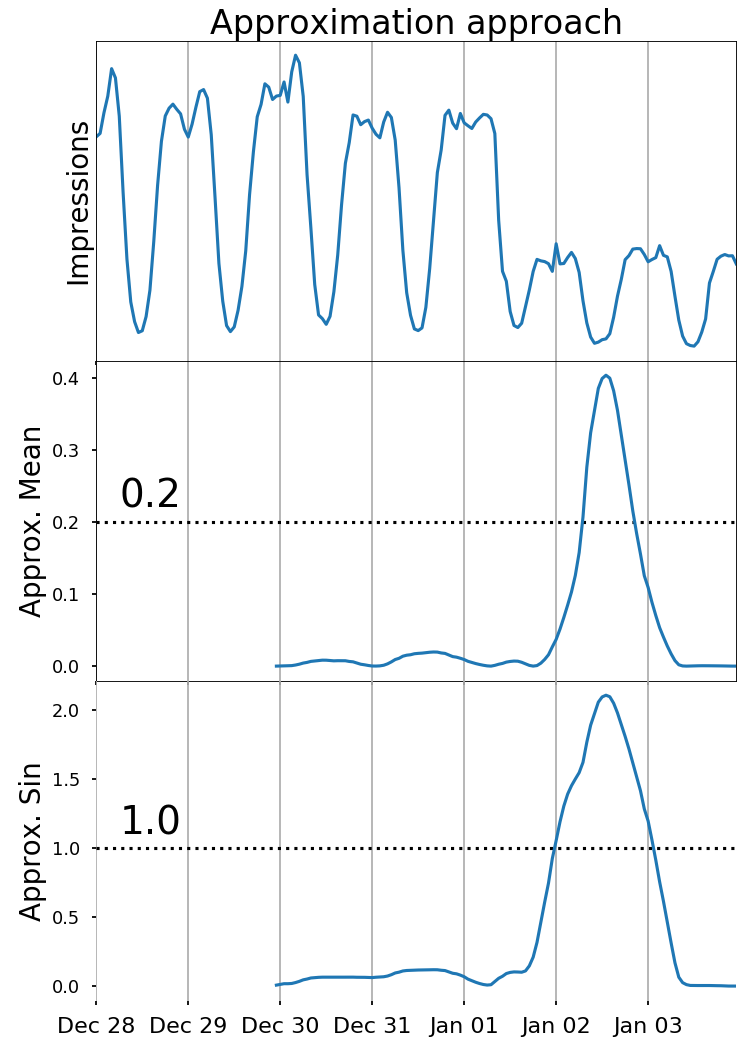
\includegraphics[height=6cm]{images/methods_comparison_1_2}
	\end{figure}
	
     \end{columns}
 
 \medskip    
     \hfill Approximation approach is better

\end{frame}


\begin{frame}
    \frametitle{Applications to real data. Mean change}
  \begin{columns}[T,onlytextwidth]
      \column{0.5\textwidth}
\begin{figure}
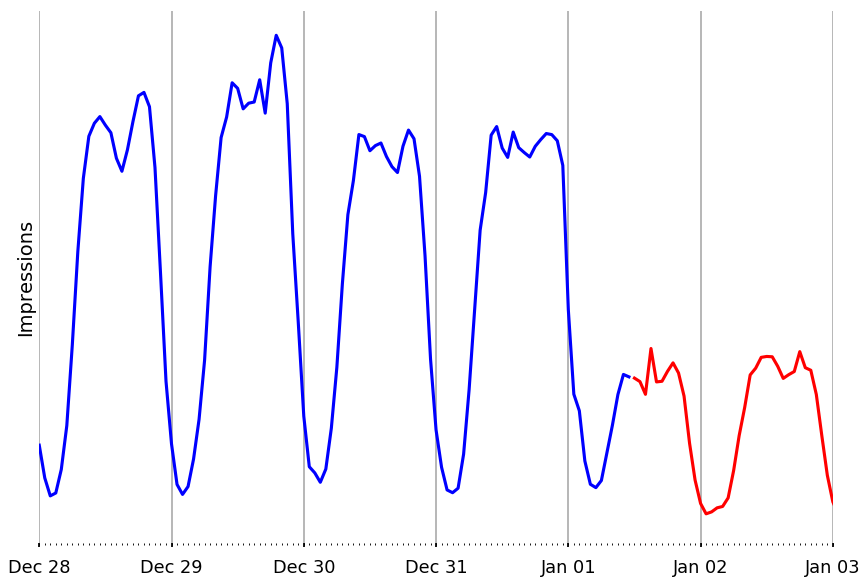
\includegraphics[scale=0.2]{images/methods_comparison_2}
\end{figure}
      \column{0.5\textwidth}
	    \begin{itemize}
	    \item Approximation-based approach
        \item Model with constant trend and daily oscillations
        \item Threshold = 1
	    \end{itemize}
     \end{columns}
\end{frame}



\begin{frame}
    \frametitle{Applications to real data. Outlier}
  \begin{columns}[T,onlytextwidth]
      \column{0.5\textwidth}
	\begin{figure}
	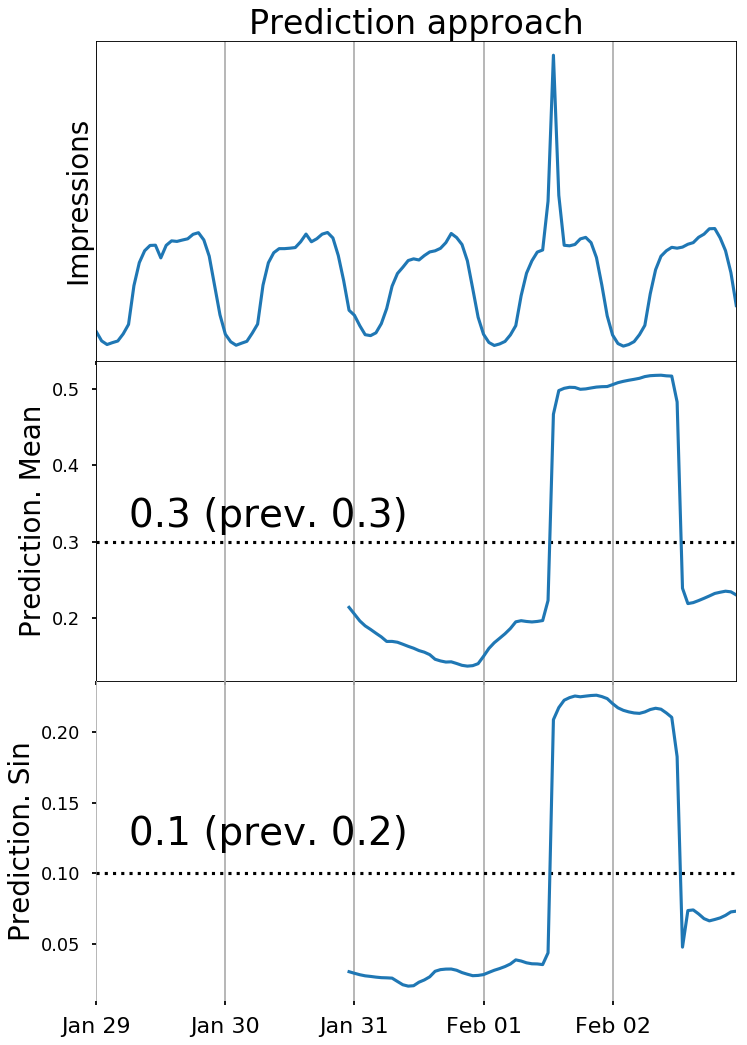
\includegraphics[height=6cm]{images/methods_comparison_2_1}
	\end{figure}
	
      \column{0.5\textwidth}
	\begin{figure}
	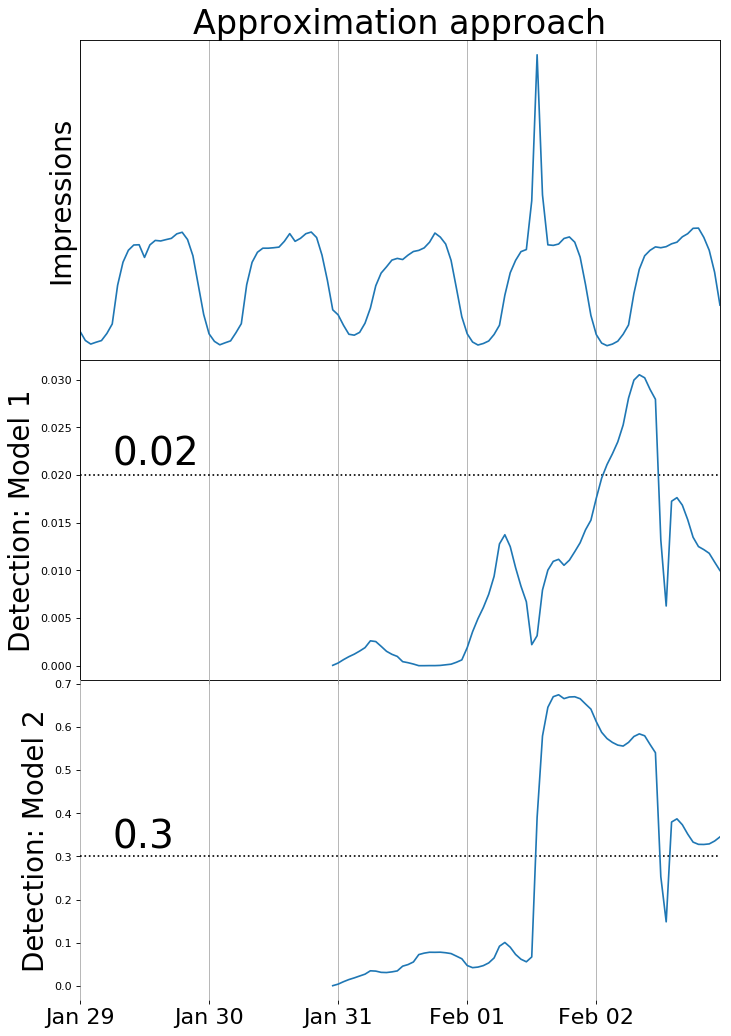
\includegraphics[height=6cm]{images/methods_comparison_2_2}
	\end{figure}
	
     \end{columns}
     
 \medskip
    \qquad Prediction approach is better

\end{frame}

\begin{frame}
    \frametitle{Applications to real data. Outlier}
  \begin{columns}[T,onlytextwidth]
      \column{0.5\textwidth}
	\begin{figure}
	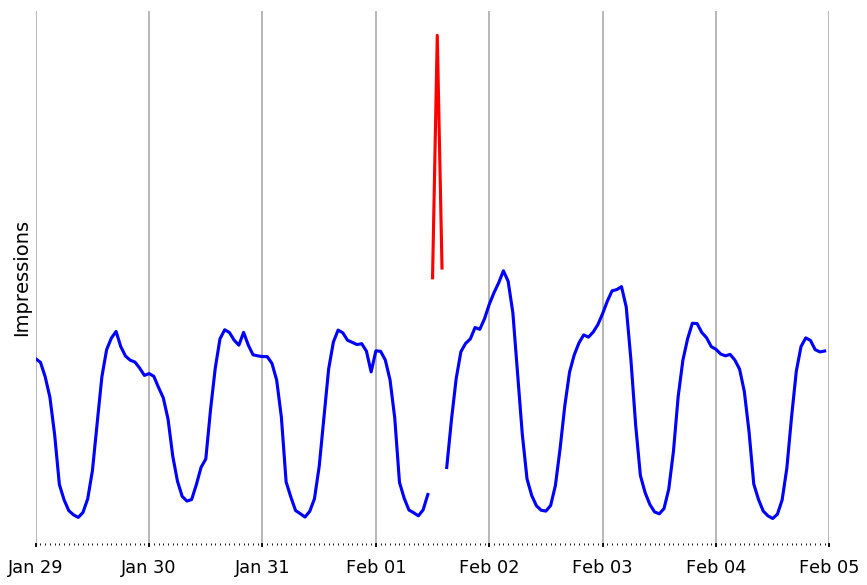
\includegraphics[scale=0.2]{images/methods_comparison_4}
	\end{figure}
      \column{0.5\textwidth}
	    \begin{itemize}
	    \item Prediction-based approach 
        \item Model with constant trend
        \item Threshold = 0.1
	    \end{itemize}
     \end{columns}

\end{frame}


\begin{frame}
    \frametitle{Applications to real data. Discussion}

%\begin{table}
%\centering
%Models thresholds
%\begin{tabular}[t]{|p{8em}|p{5em}|p{5em}|p{5em}|p{5em}|}
%\hline
%  & Pred. Mean & Pred. Sin & Approx. Mean & Approx. Sin\\
%\hline
%Change in mean & 0.3 (0.25 - 0.35) & 0.2 (0.05 - 0.35) & 0.2 (0.01 - 0.4) & 1.0 (0.01 - 2.0)\\
%\hline
%Local change (outlier) & 0.3 (0.2 - 0.5) & 0.1 (0.05 - 0.2) & 0.02 (0.01 - 0.03) & 0.3 (0.01 - 0.6)\\
%\hline
%%Change in periodic component & 0.26 (0.22 - 0.30) & 0.05 (0.04 - 0.07) & 0.005 (0.001 - 0.010) & 0.05 (0.01 - 0.12)\\
%%\hline
%\end{tabular}
%\end{table}

\begin{itemize}
	\item Different methods should be chosen for different types of change points. Prediction-based approach looks more perspective for outliers prediction, whereas Approximation-based approach is more robust for changes in mean. 
\bigskip
	\item Model with constant trend finds change points well, despite of clear daily oscillations. However, in more complex cases, it is important to choose a proper model. E.g., the model with constant trend is totally inappropriate for the case of linear trends.
\bigskip
	\item Choice of thresholds is a big challenge. Moreover, for different types of change points,
threshold can be different. 
\end{itemize}

\end{frame}

\begin{frame}
    \frametitle{Direction of CP search}
We can search for change points in different directions
\begin{itemize}
	\item Forward (always from left to right). Good for alerts.
\medskip
	\item Backward (always from right to left). Good for forecast.
\medskip
	\item Both forward and backward to localize the change interval. Good for analysis of historical data.
\end{itemize}

\smallskip
  \begin{columns}[T,onlytextwidth]
      \column{0.5\textwidth}
      Forward method:
	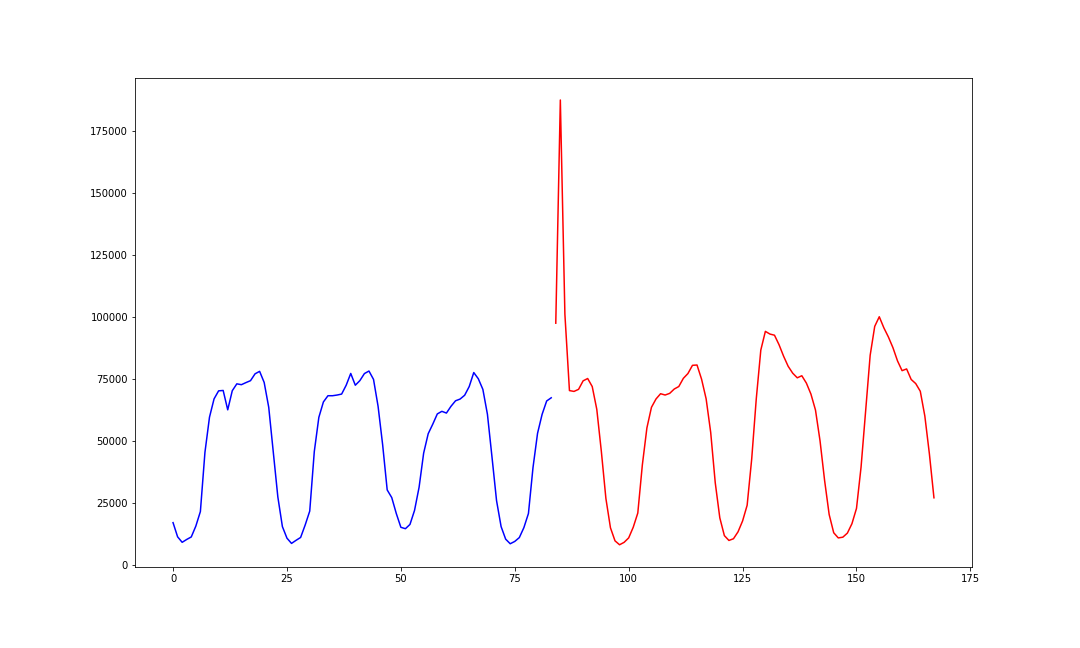
\includegraphics[scale=0.15]{images/022_point_cp_detected}
      \column{0.5\textwidth}
      Forward-backward method:
      
      \vspace*{0.3cm}
	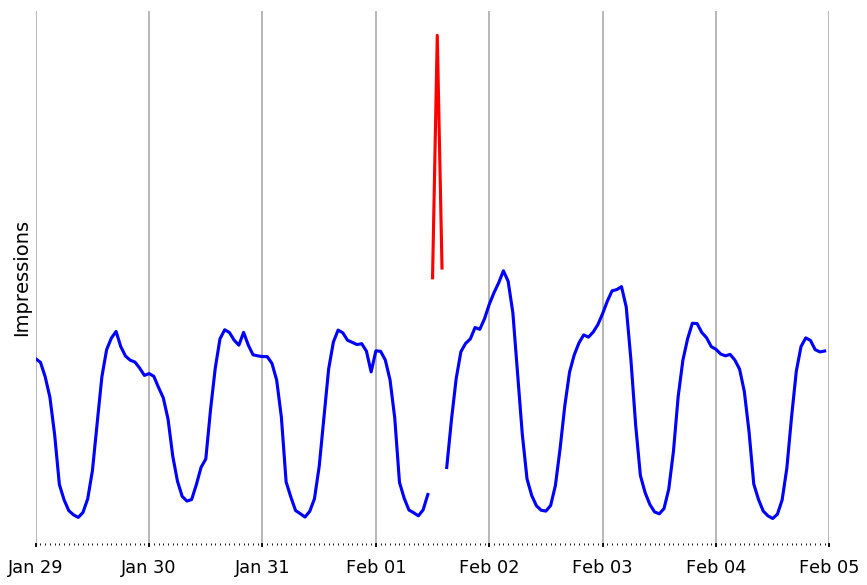
\includegraphics[scale=0.15]{images/methods_comparison_4}
     \end{columns}


\end{frame}

\begin{frame}
    \frametitle{Applications to real data. Long time series}
    
\textblue{Final model}: Approximation-based approach with the model with constant trend, threshold = 0.4 and forward-backward search method.

\bigskip
Two different countries
\medskip
  \begin{columns}[T,onlytextwidth]
      \column{0.5\textwidth}
	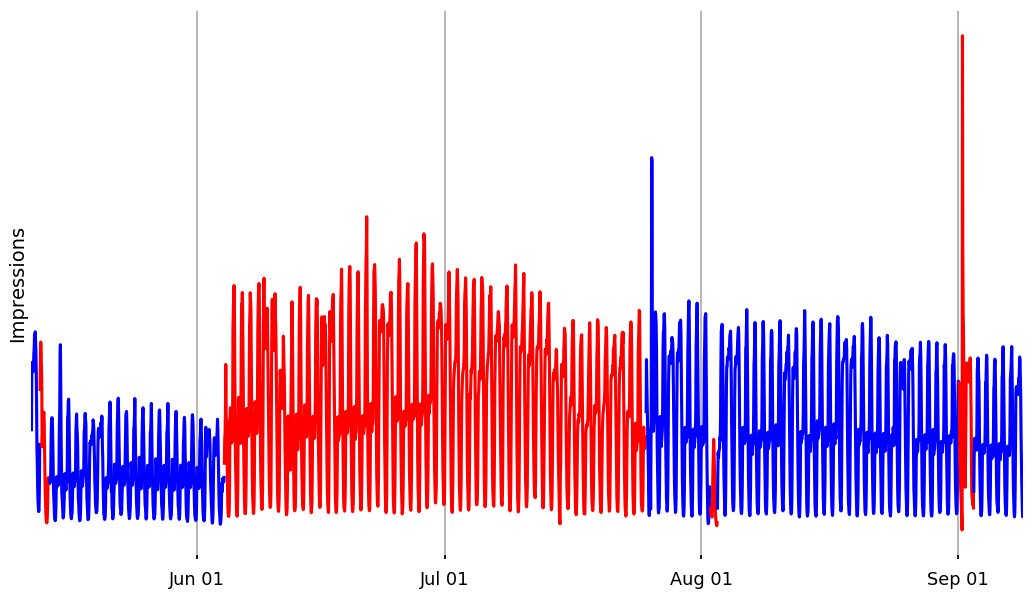
\includegraphics[scale=0.16]{images/long_ts_1}
      \column{0.5\textwidth}
	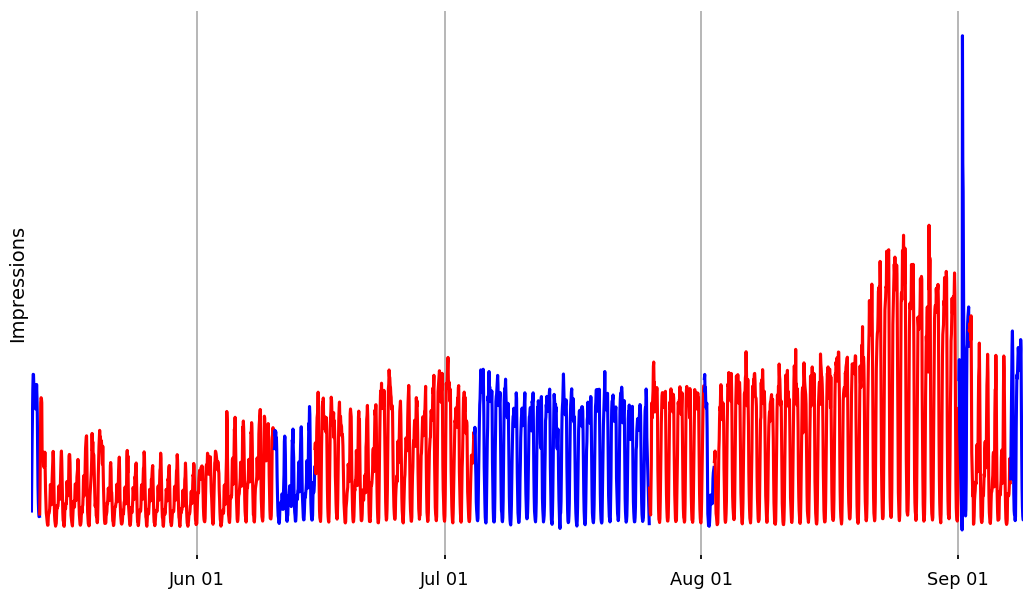
\includegraphics[scale=0.16]{images/long_ts_2}
     \end{columns}
\end{frame}


% \begin{frame}
%    \frametitle{What about trend change?}

% Above models don't really work here:

%   \begin{columns}[T,onlytextwidth]
%       \column{0.5\textwidth}
% 	\begin{figure}
% 	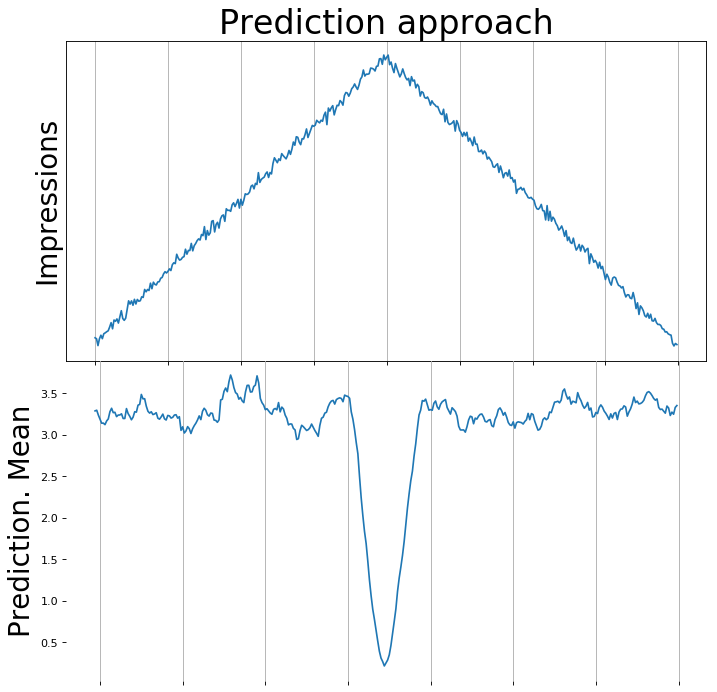
\includegraphics[height=5.5cm]{images/methods_comparison_4_1}
% 	\end{figure}
	
%       \column{0.5\textwidth}
% 	\begin{figure}
% 	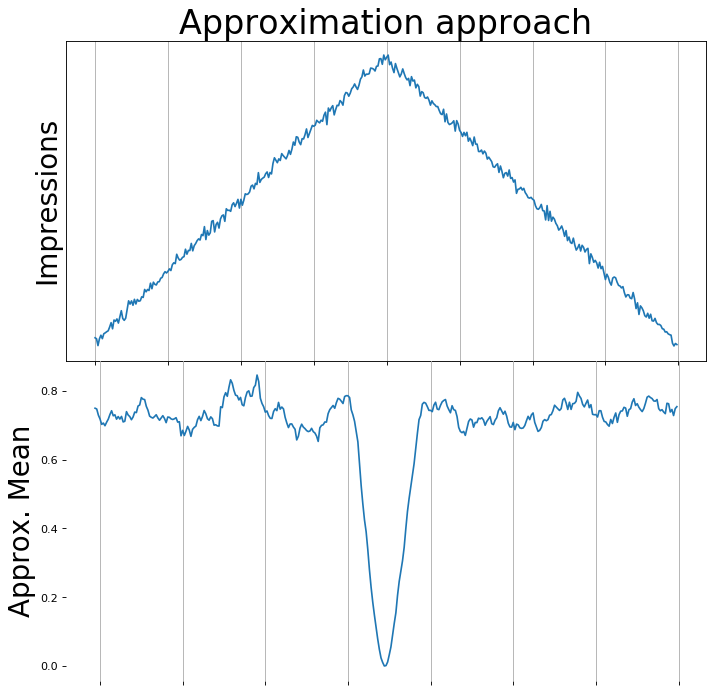
\includegraphics[height=5.5cm]{images/methods_comparison_4_2}
% 	\end{figure}
	
%      \end{columns}

% \end{frame}

% \begin{frame}
%     \frametitle{Model for trend change detection}


% We can just add linear trend part (B) to our model:
% $$ \mathrm{X} = a + Bn + C\cos(2\pi \frac{n}{24}) + S \sin(2\pi \frac{n}{24}) + \epsilon $$

% \begin{figure}
% 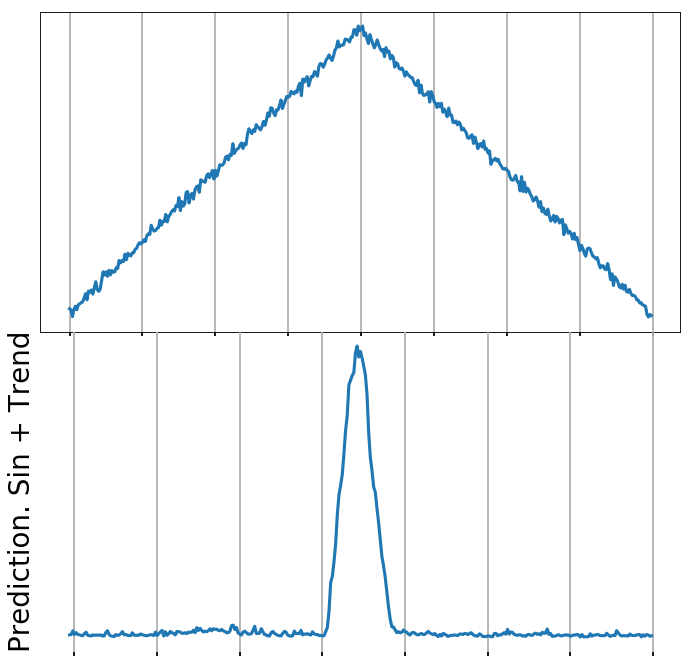
\includegraphics[scale=0.25]{images/methods_comparison_5_1}
% \end{figure}

% To allocate trend change we can aggregate data on daily level. Then apply change point detection with linear regression (as an example) model
% \end{frame}


\begin{frame}
    \frametitle{Approaches to model and threshold choice}

\begin{enumerate}
\item 
Theoretical approach based on the model of data. Drawback: usually, real-world data are various and do not fit a model exactly.

\bigskip
\item
Supervised machine-learning approach when data are tagged in advance and then learning is performed by comparison of found change points and tagged change points. Drawback: it is a hard task to tag the data in advance.

\bigskip
\item
Empirical approach with adaptive adjustment of the threshold. This is a very promising method:
each alert is considered by business people from the viewpoint of its
importance. If there are too many false alerts, then threshold increases. 
\end{enumerate}

%Supervised machine learning techniques can be applied if the data are tagged by change-points.
%\newline
%
%We can estimate parameters mentioned above compare quality of change point detection using cross validation.
%\newline
%Quality can be estimated as sum of distance between real indexes and estimated indexes normalized by length of time series: $$\sum_{i=1}^K \frac{|\widehat{t_i} - t_i|}{N}$$	
%
%It works perfectly, when our time series is tagged with change points.

 \end{frame}

%\begin{frame}
%    \frametitle{Machine learning for parameters estimation}
%
%In real world there is no objectively good or bad tagging in this problem. So sometimes it is hard to tag the time series.
%
%\begin{figure}
%\includegraphics[scale=0.2]{images/examples_tagging}
%\end{figure}
%
%The possible solutions:
%	    \begin{itemize}
%	    	\item Tag it accordingly to what's important for business
%		\item Estimate quality on higher level of task
%	    \end{itemize}
%
% \end{frame}
%


\begin{frame}
    \frametitle{Airpush experience}

\begin{enumerate}
  \item Alert system works at two levels:
 \begin{itemize}
	    \item Hourly level model, which detect local changes in mean, variance, daily oscillations and detects anomalies
		\item Daily level model, which detect changes in global trend
\end{itemize}
\bigskip
\item
Overall impressions data are splitted by countries, ad formats, applications,
since the sources of changes can be specific for these characteristics. 
%Applying described methods can help us to identify change points automatically in every big enough %country/applications/application/ad format time series.
\bigskip
\item
Thresholds are adjusted adaptively by monitoring for false alerts.
\end{enumerate}

\end{frame}

\begin{frame}
    \frametitle{Next steps}

But we can move forward. 
Instead of plain alerts we can develop \textblue{smart alert system}:\\

Instead of sending notification on each separate case (which could be a lot of at once), the system aggregates alerts and send you only a summary.

\bigskip
Example:

\medskip
 \begin{itemize}
	    \item Countries: 167 out of 196 had change
		\item Ad formats: 6 out of 8 had change
		\item Applications: 1 out of 3000 had change
\end{itemize}

\medskip
 This example means that something affected almost all countries and almost all ad formats, \textbf{but} only one application. That is why most probably real root of change is the application, so we want to be notified only about this application.

\end{frame}


\begin{frame}
    \frametitle{Conclusion}

	    \begin{itemize}
	    \item Change point detection system can help us to react on significant change fast.

\bigskip
		\item The important application is the alert system. However,  the scope of applications 
is much wider.

\bigskip
		\item The model of time series should be chosen adequately to the data and the changes to detect.

\bigskip
        \item The problem of threshold choice is sophisticated. However, if the model is chosen adequately,
        the choice of threshold can be performed adaptively on the base of false alerts. 	    \end{itemize}

 \end{frame}


% \begin{frame}
%     \frametitle{Conclusion}

% 	    \begin{itemize}
% 	    	\item Main approaches works well on the real data and are good for different applications
% 		\item Wisely choosing of applicable model is important
% 		\item We can choose threshold which applicable to our task
% 		\item Aggregation of periods can help to find more general changes
% 		\item Change point detection system can help us to react on significant change fast
% 		\item Accurate tagging will allow to estimate detection quality
% 	    \end{itemize}

%  \end{frame}


\end{document}
